\documentclass[12pt]{article}
\usepackage{graphicx} % Required for inserting images
\usepackage{graphicx}
\usepackage{caption}
\usepackage{subcaption}
\usepackage{enumitem}
\usepackage[margin=3.5cm]{geometry} 
\usepackage{amsmath,amsthm,amssymb}
\usepackage{hyperref}
\usepackage[mathscr]{euscript}
\usepackage{xcolor} 
\usepackage{calrsfs}
\usepackage{sectsty}
\usepackage{amsmath}
\usepackage{amsthm}
\newcommand*{\mybox}[1]{\framebox{#1}}
\sectionfont{\centering}
% \usepackage{indentfirst}
\begin{document}
\begin{figure}
\centering

\includegraphics[width=5.5cm,scale=2.5]{logo.jpg}
\label{fig:cenario}
\end{figure}
\vspace{-40pt}
\title{\textbf{Electronic Design Lab}\\
\vspace{10pt}
Milestone -2\\
\vspace{10pt}
\textbf{Schematic and preliminary analysis review}}
\author{
  Mohit Jindal \\
  \texttt{20D070052}
  \and
  Vinayak Goyal\\
  \texttt{20D070088}
  \and
  Vrinda Goel\\
  \texttt{20D070090}
}


\maketitle
\newpage

%---------------------------------------------------------------------------------------------------------------------------------------------------------------------
% \title{EE344-EDL REPORT}
% \author{Vrinda Goel}
% \date{February 2023}


\newpage
\maketitle

\section{PCB Schematics}

Given Below are the PCB Schematics for our PCR Machine. These include the Schematic for Micro-controllers, H-Bridge, Voltage Regulator, Power Supply, Sensors Connection, etc.\\

Given Below is the pin allotment that we have made:\\
\begin{itemize}
    \item \textbf{ADCs}: We have used 2 inbuilt ADCs for 2 thermistors, one for the temperature of peltier and other for the temperature of heated lid. Pins PA0 and PA1 are used as input pins for these ADCs. We could have used the pins PA0-PA7 and PB0-PB1 as analog pins for this purpose.

    \item \textbf{LCD}: We have used GPIO Pins(General Purpose Input Output) for this. There are a total of 37 GPIO pins in out micro-controller. We have alloted pins A6-A7, B0-B1 and B10-B11 as the output pins for LCD Display. This will basically be the temperature display of ADC output.

    \item \textbf{Fan}: A PWM Pin is allocated to control whether the Fan will be ON/OFF. It will be ON when we want to cool the system otherwise it will be OFF. The Pin allocated for this is PB6 which is PWM signal.

    \item \textbf{H-Bridge}: We have used PWM Pins for this. There are 15 PWM Pins in our micro-controller which are PA0-PA3, PA6-PA10, PB0-PB1 and PB6-PB9. In our schematic we have used PA8-PA10 PWM Pins as input to the H-Bridge. The output of H-Bridge is given to the peltier through OUTA-OUTB and a CS(Current Sensor) signal is sent to micro-controller through the pin PA2. 
\end{itemize}

We have made some changes in our design since the last checkpoint. We decided to integrate the PCBs of the microcontroller and H-bridge to form a single PCB. The modified PCB and the first completed layout of the PCB are shown below:

\begin{figure}[htp]
    \centering
    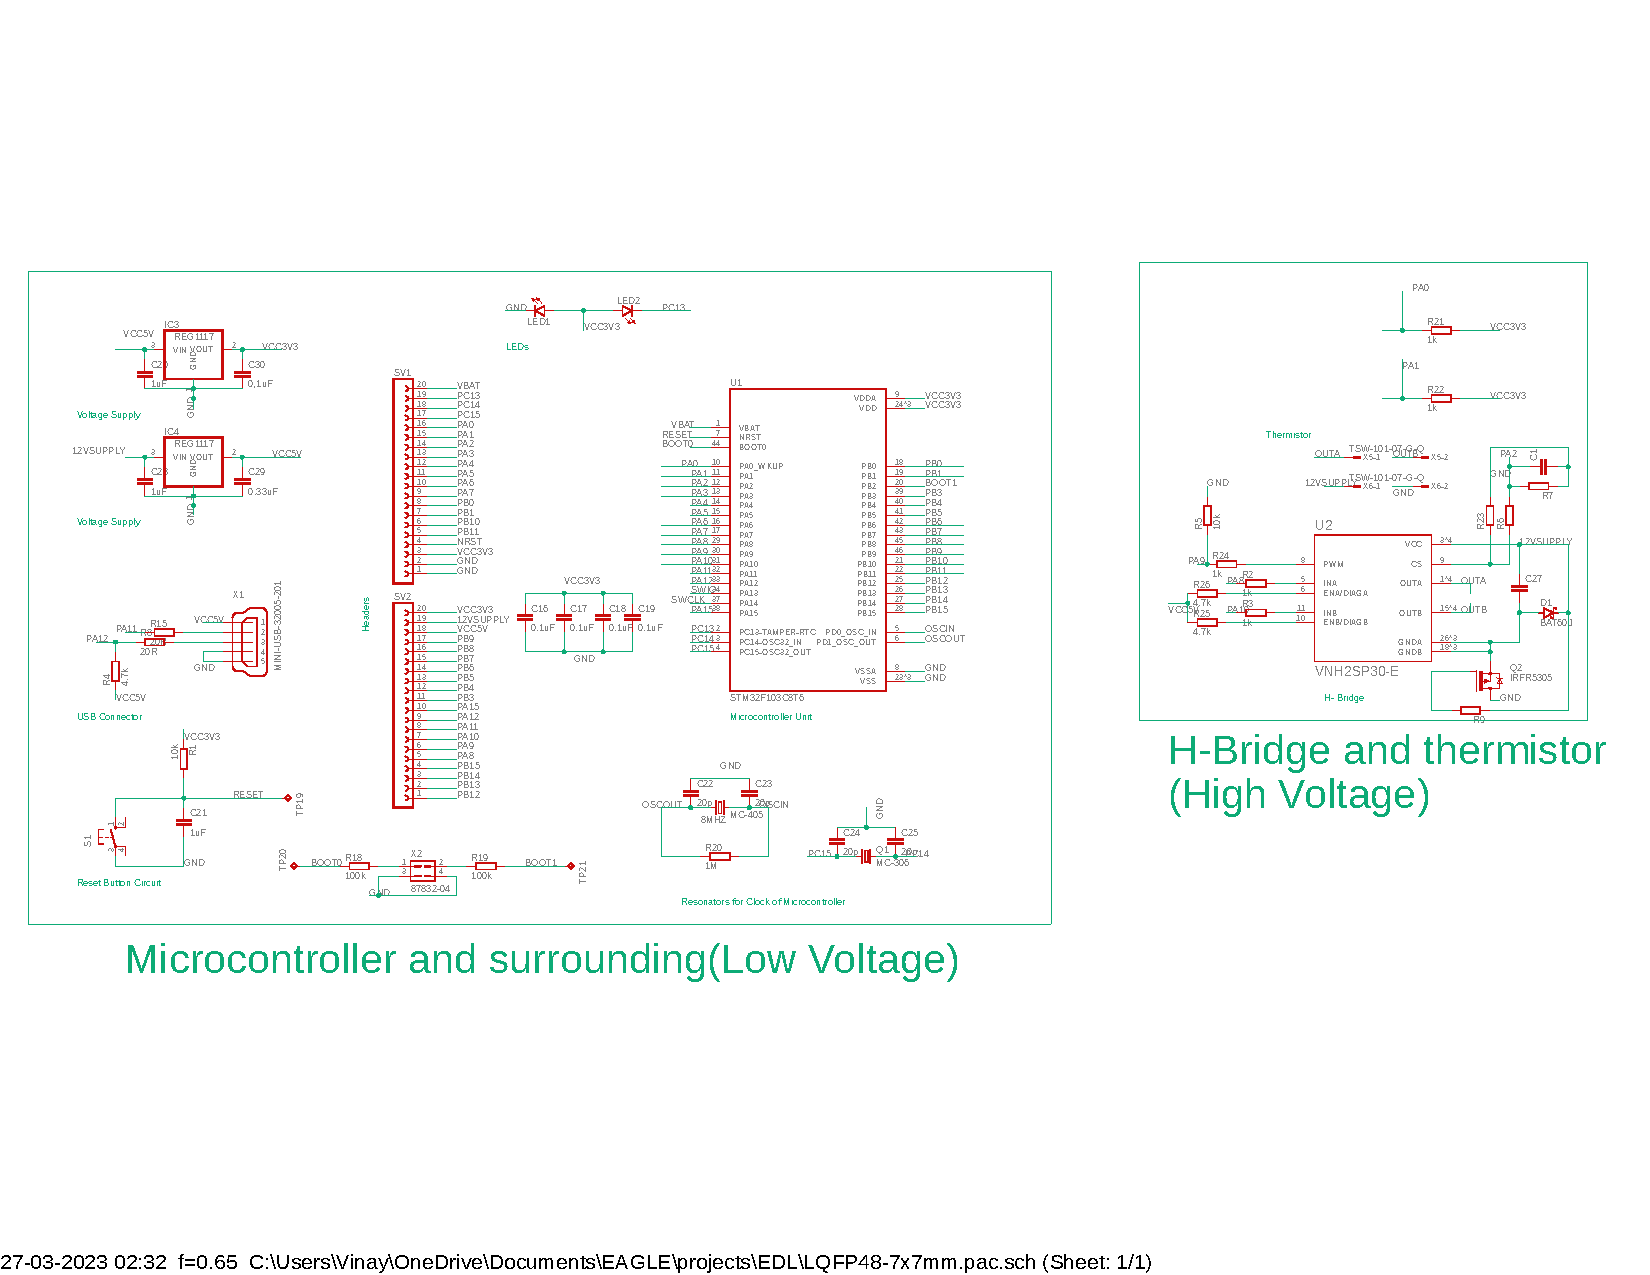
\includegraphics[width=\textwidth]{Images/ourpcbschematic.pdf}
    \caption{Schematic of our PCB}
    \label{fig:galaxy}
\end{figure}


\begin{figure}[htp]
    \centering
    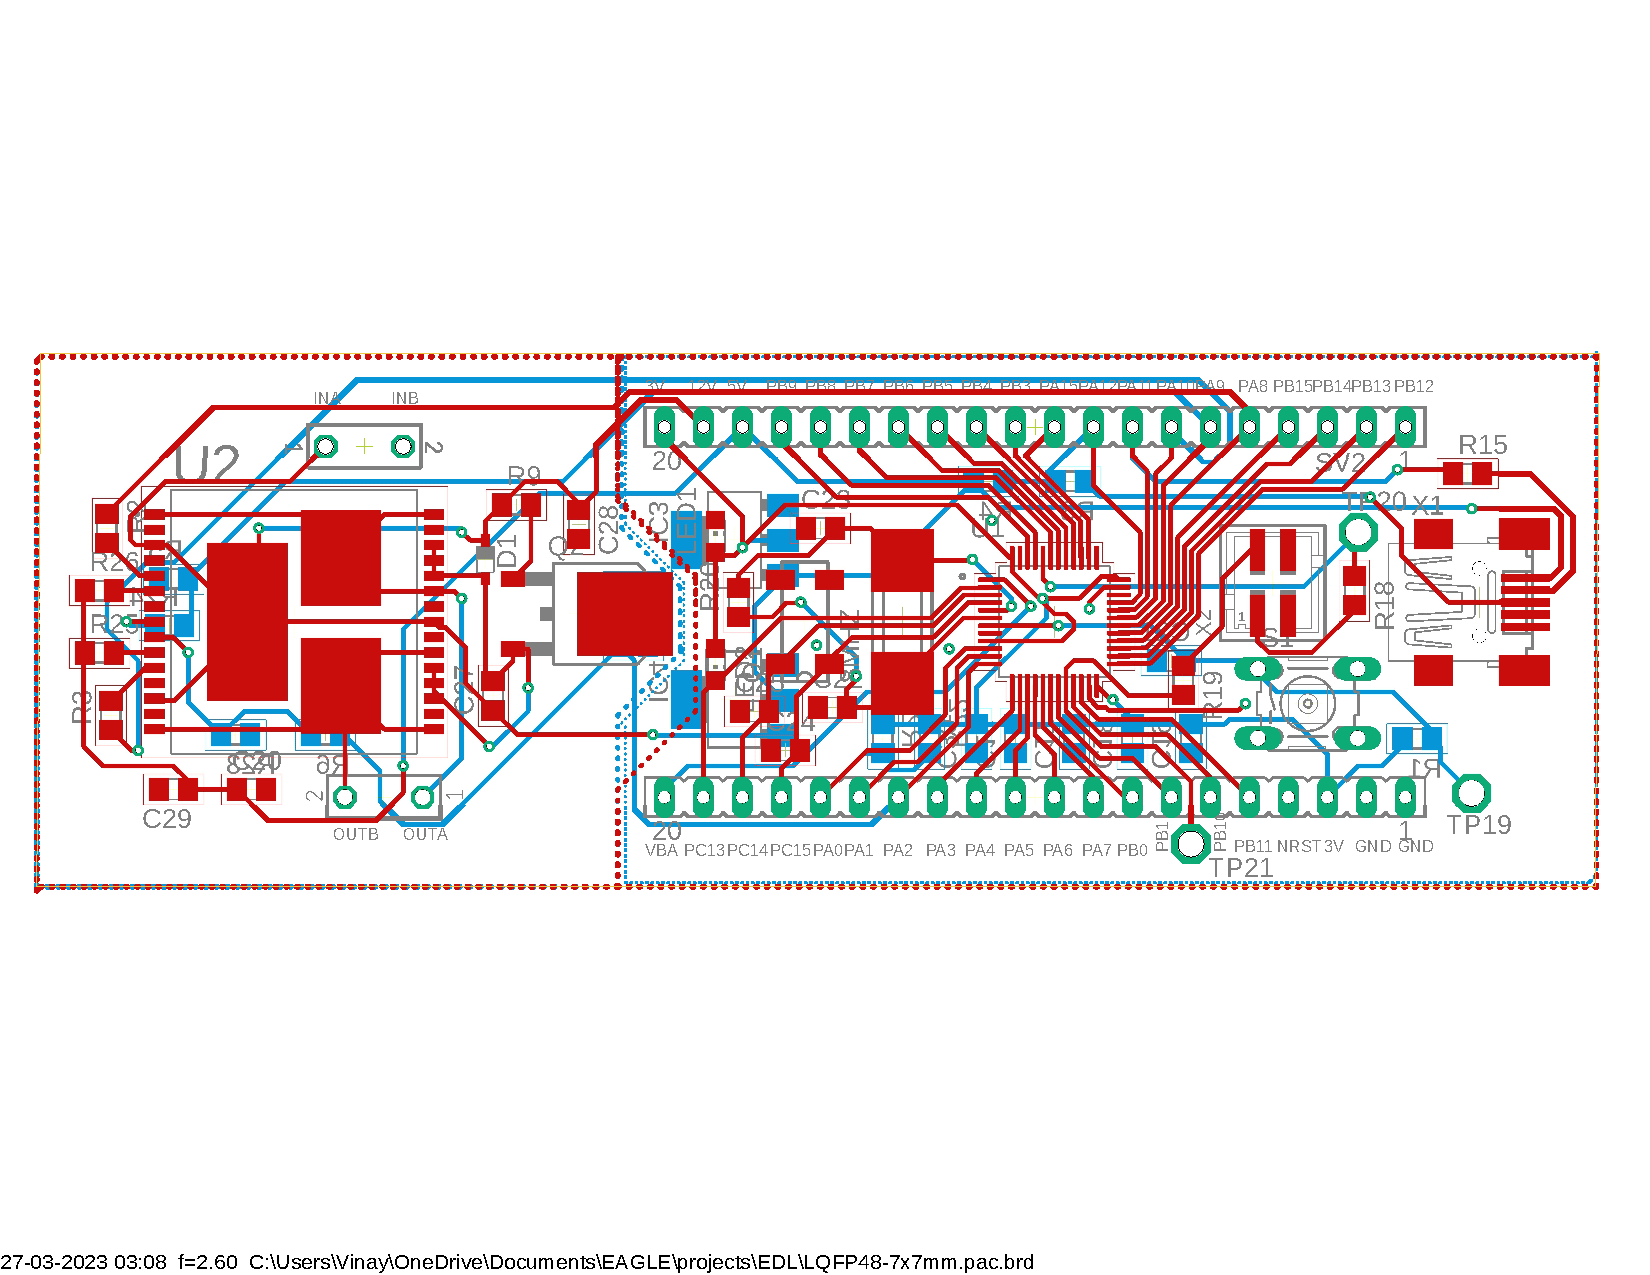
\includegraphics[width=\textwidth]{Images/ourpcbboth.pdf}
    \caption{PCB layout consisting of both layer components}
    \label{fig:galaxy}
\end{figure}


\begin{figure}[htp]
    \centering
    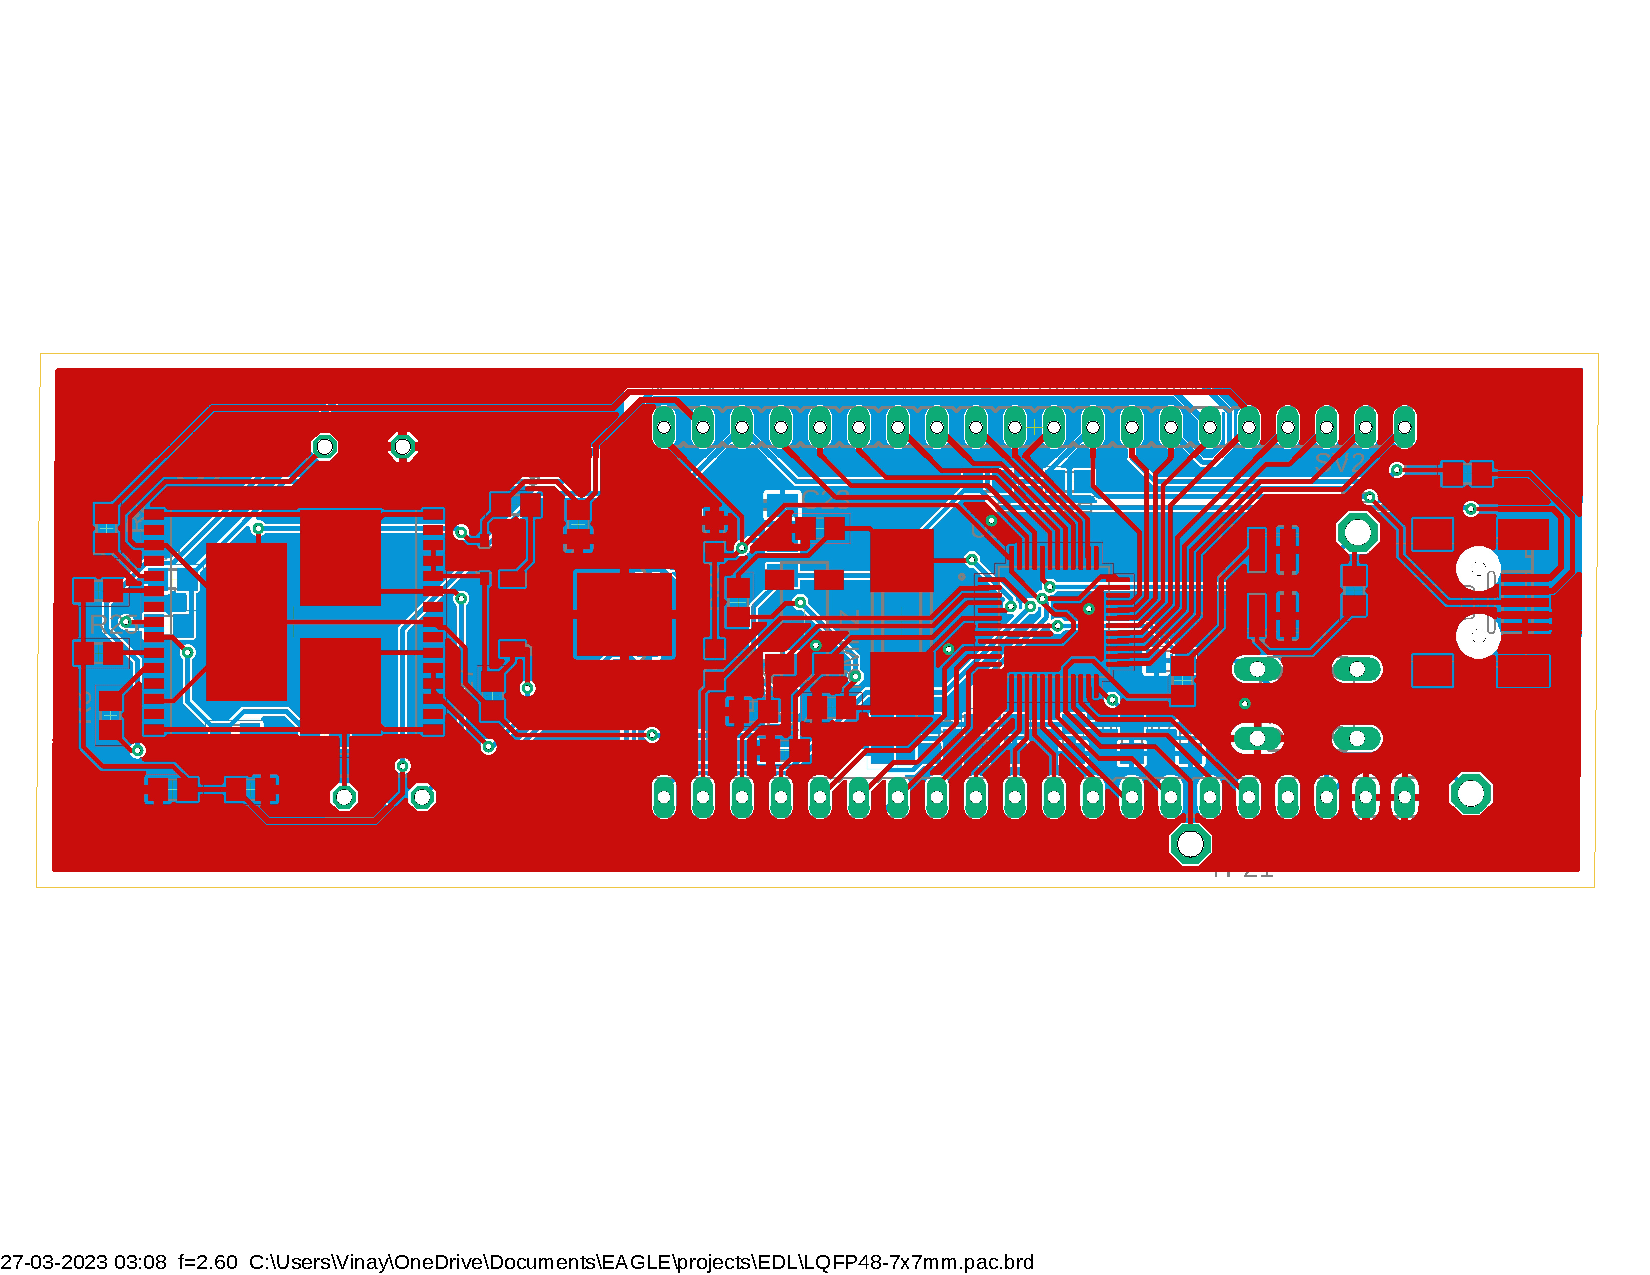
\includegraphics[width=\textwidth]{Images/ourpcbwithgplane.pdf}
    \caption{PCB layout consisting of both layer components along with ground plane}
    \label{fig:galaxy}
\end{figure}


\begin{figure}[htp]
    \centering
    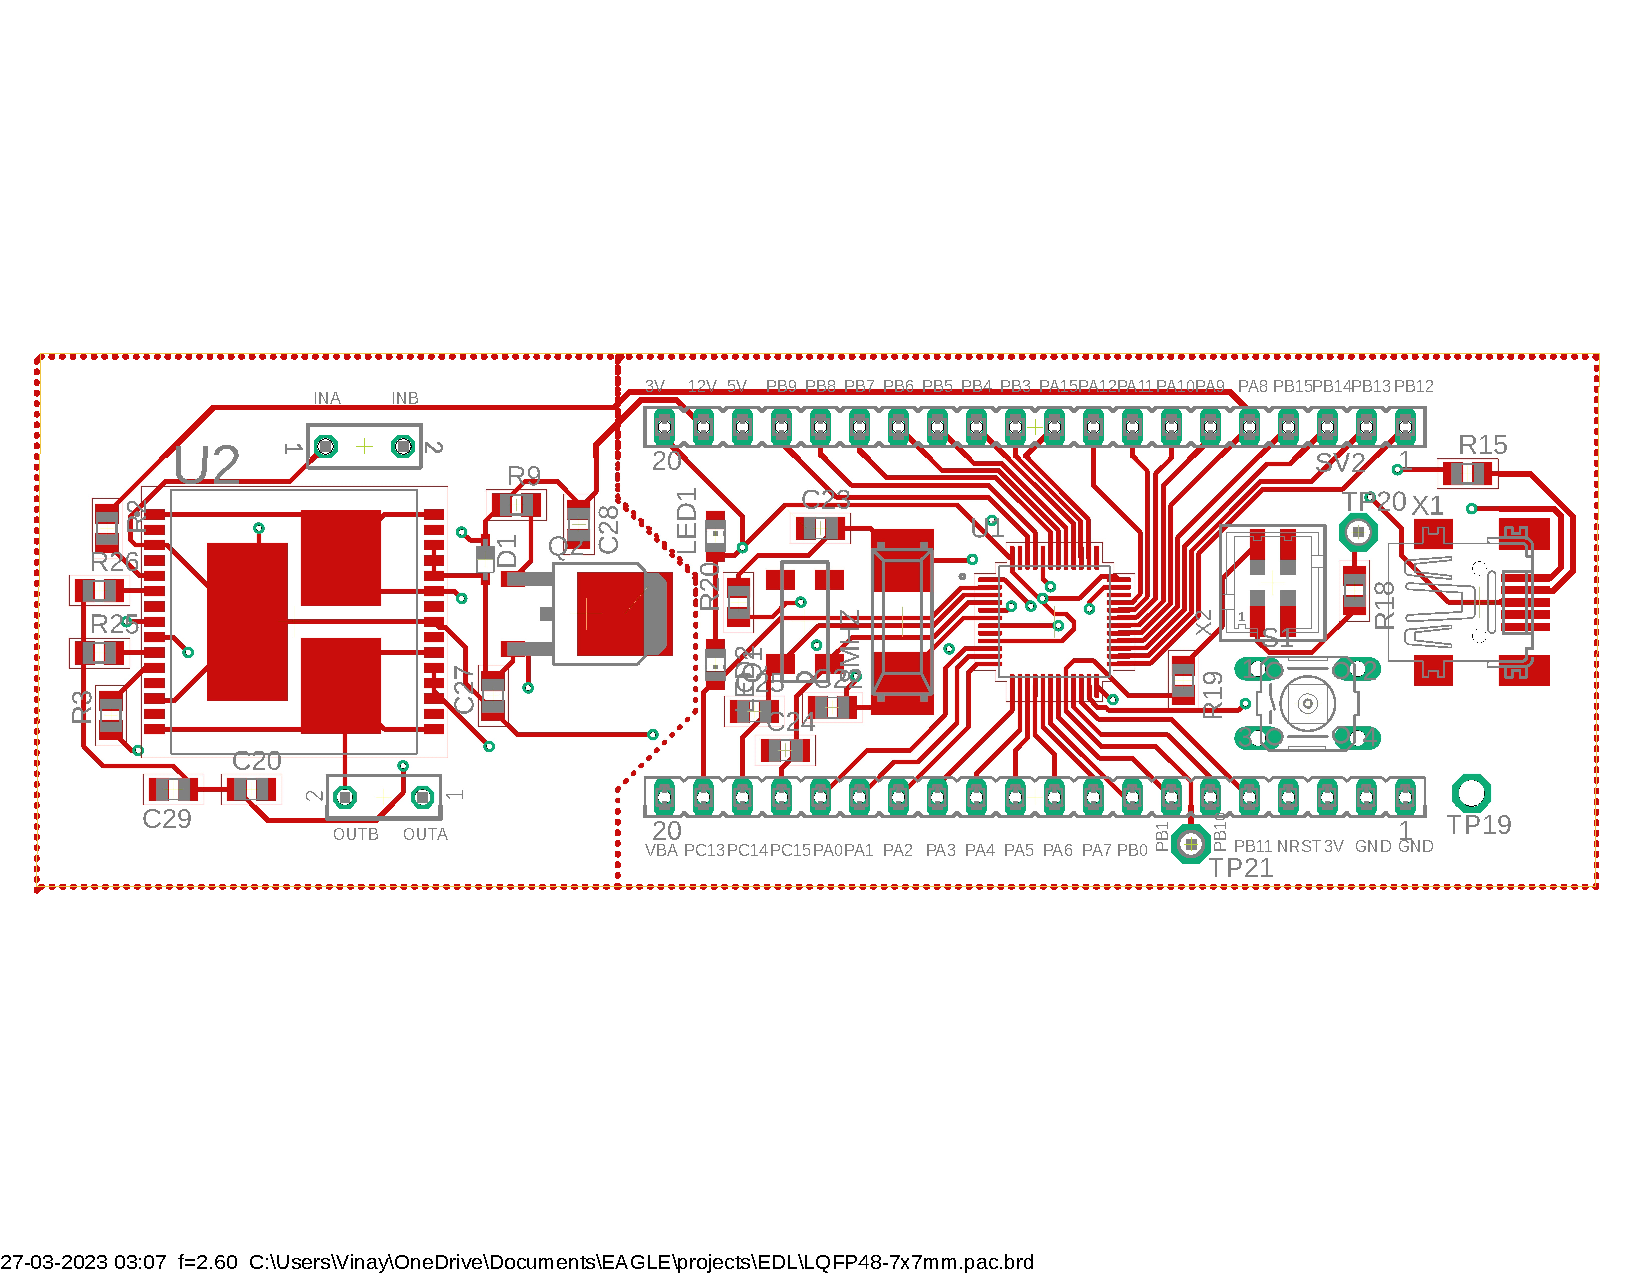
\includegraphics[width=\textwidth]{Images/ourpcbtop.pdf}
    \caption{PCB layout of the top layer}
    \label{fig:galaxy}
\end{figure}

\begin{figure}[htp]
    \centering
    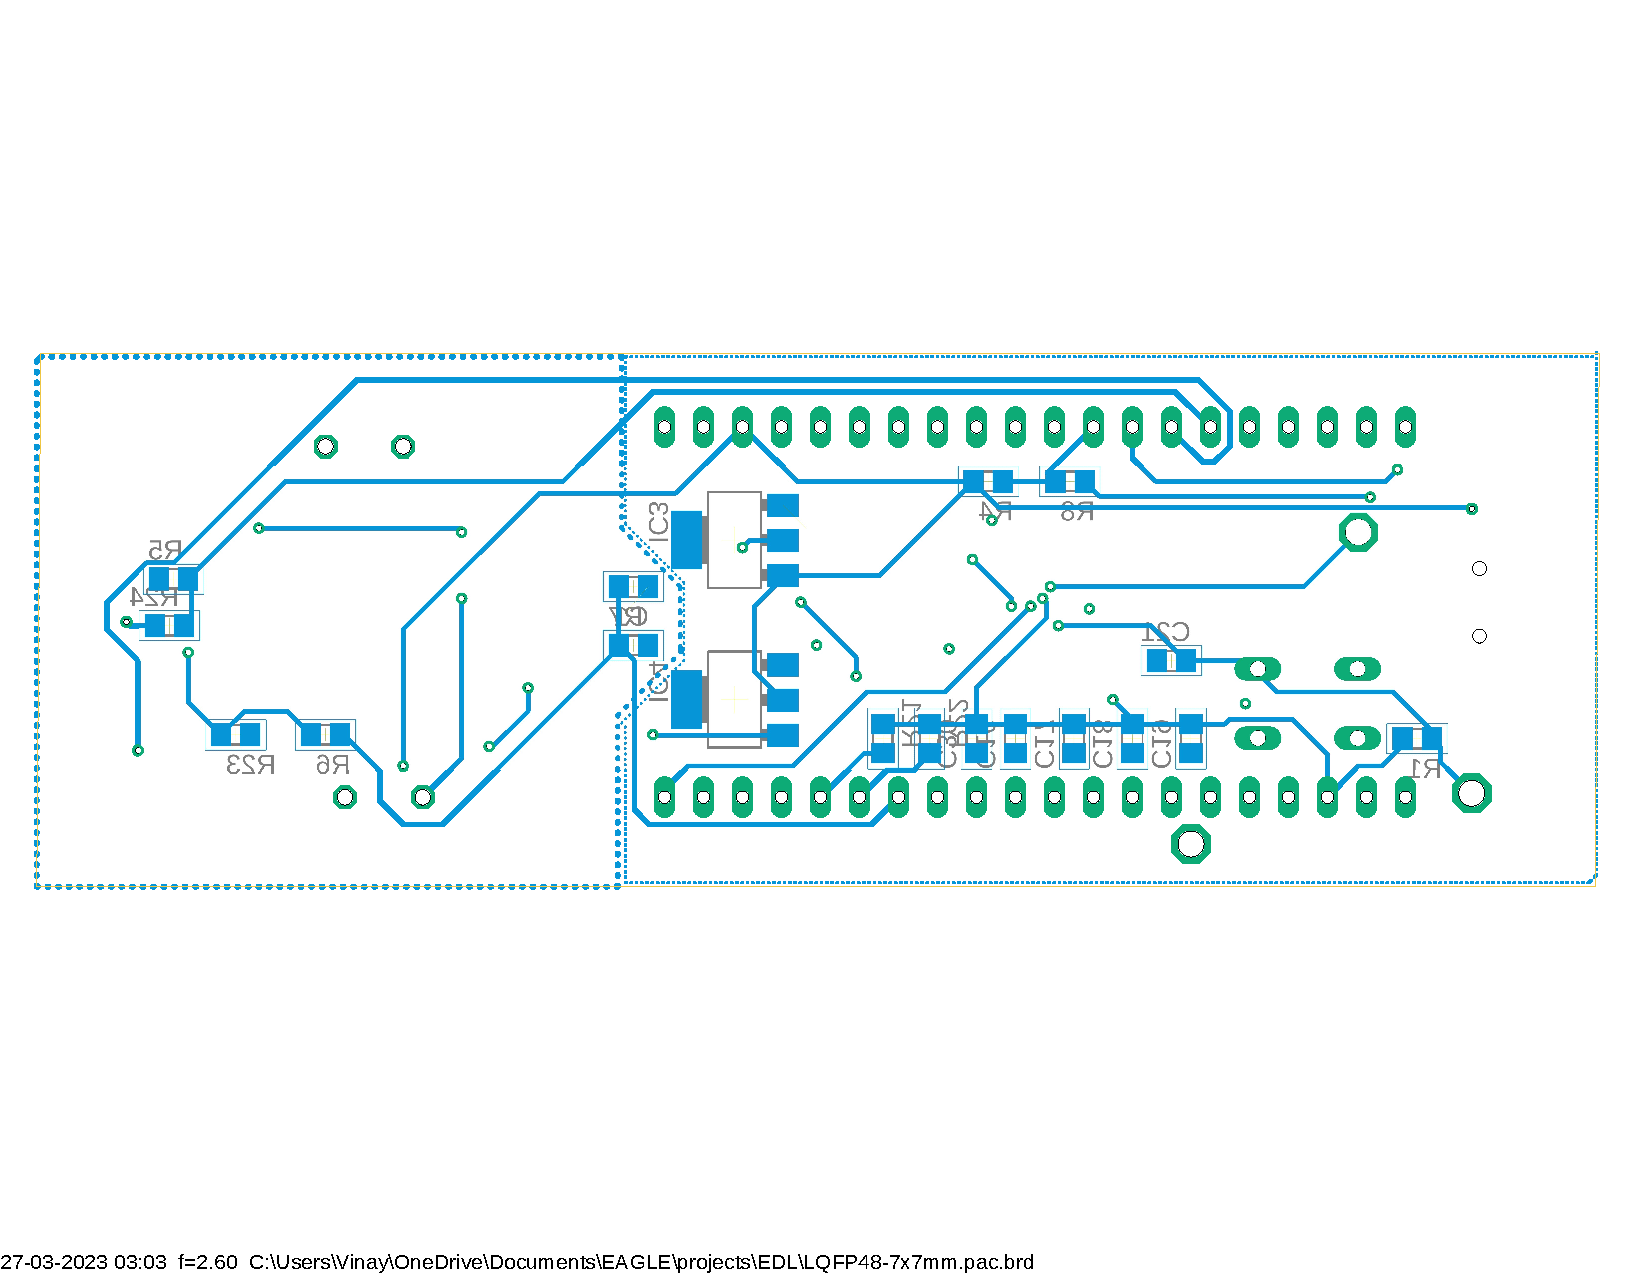
\includegraphics[width=\textwidth]{Images/ourpcbbottom.pdf}
    \caption{PCB layout of the bottom layer}
    \label{fig:galaxy}
\end{figure}

\begin{figure}[htp]
    \centering
    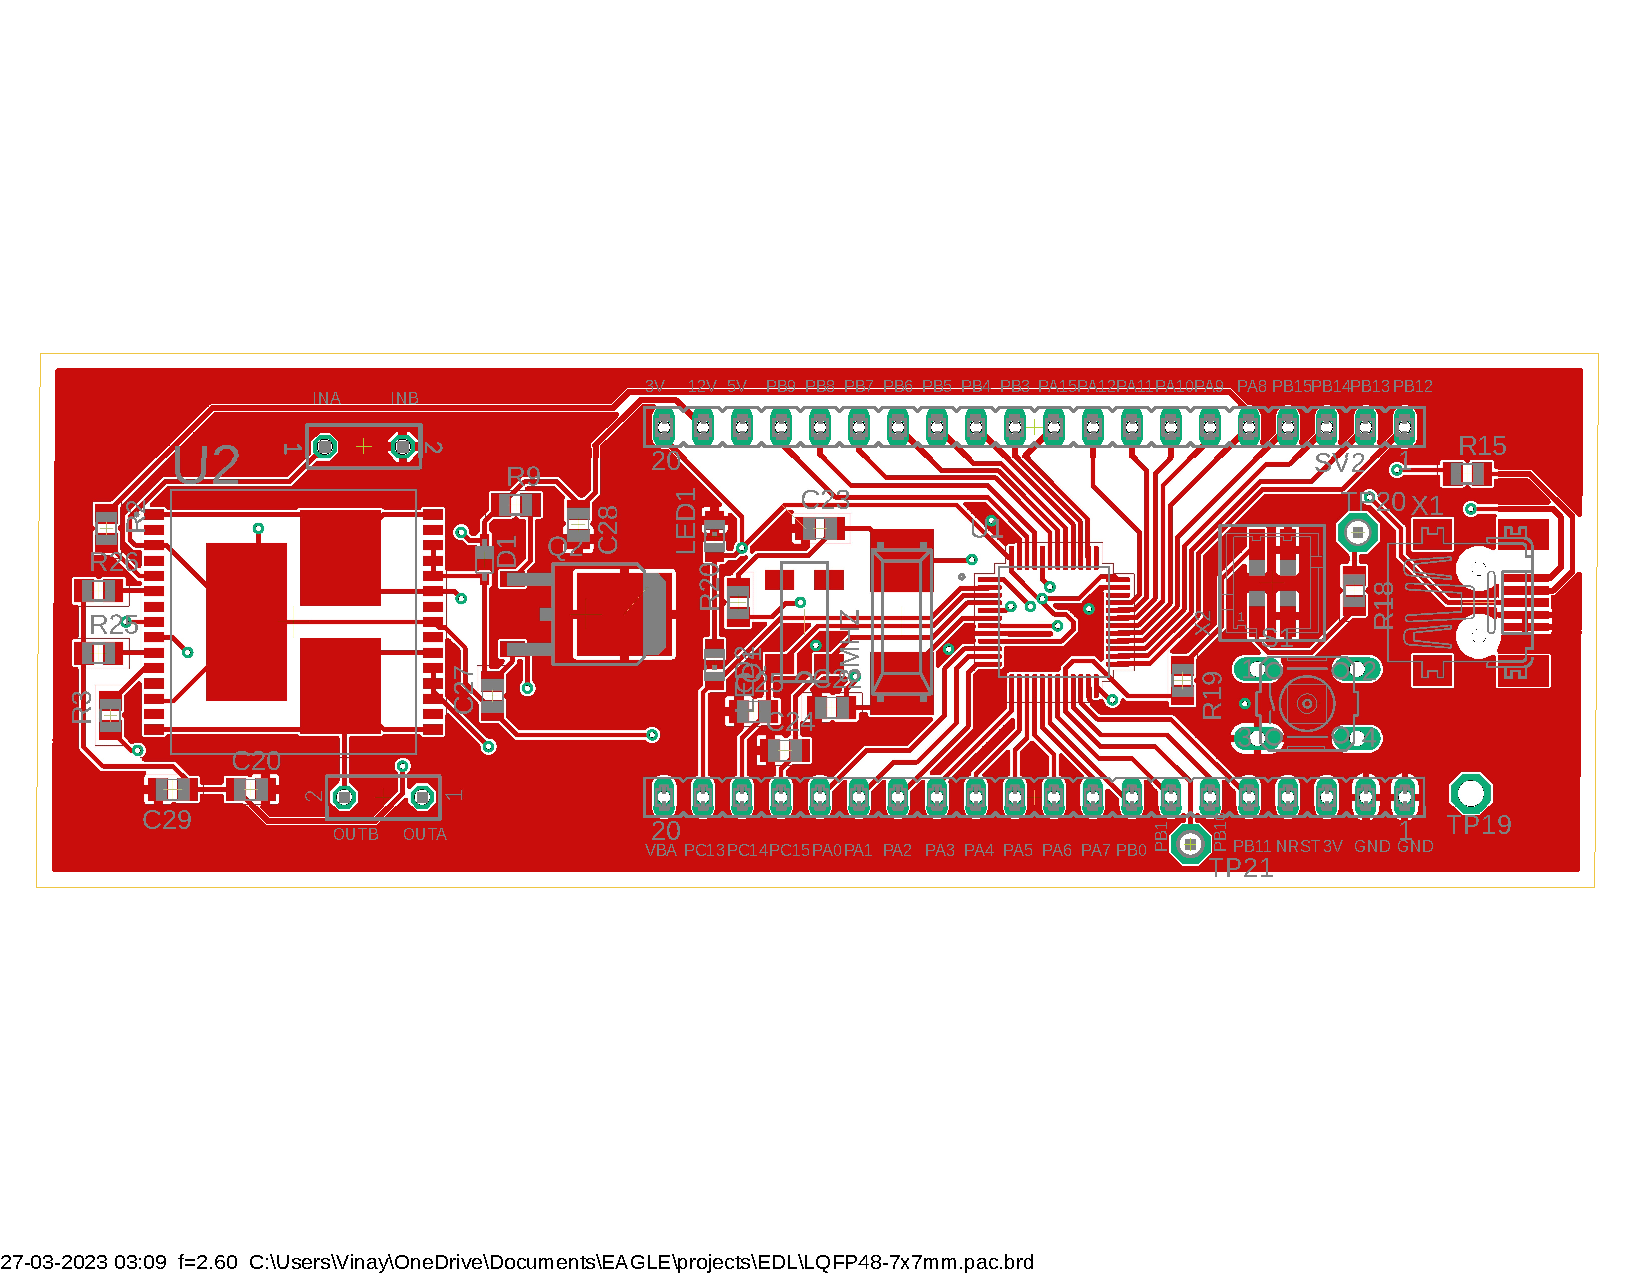
\includegraphics[width=\textwidth]{Images/ourpcbtopgplane.pdf}
    \caption{PCB layout of top layer with ground plane}
    \label{fig:galaxy}
\end{figure}

\begin{figure}[htp]
    \centering
    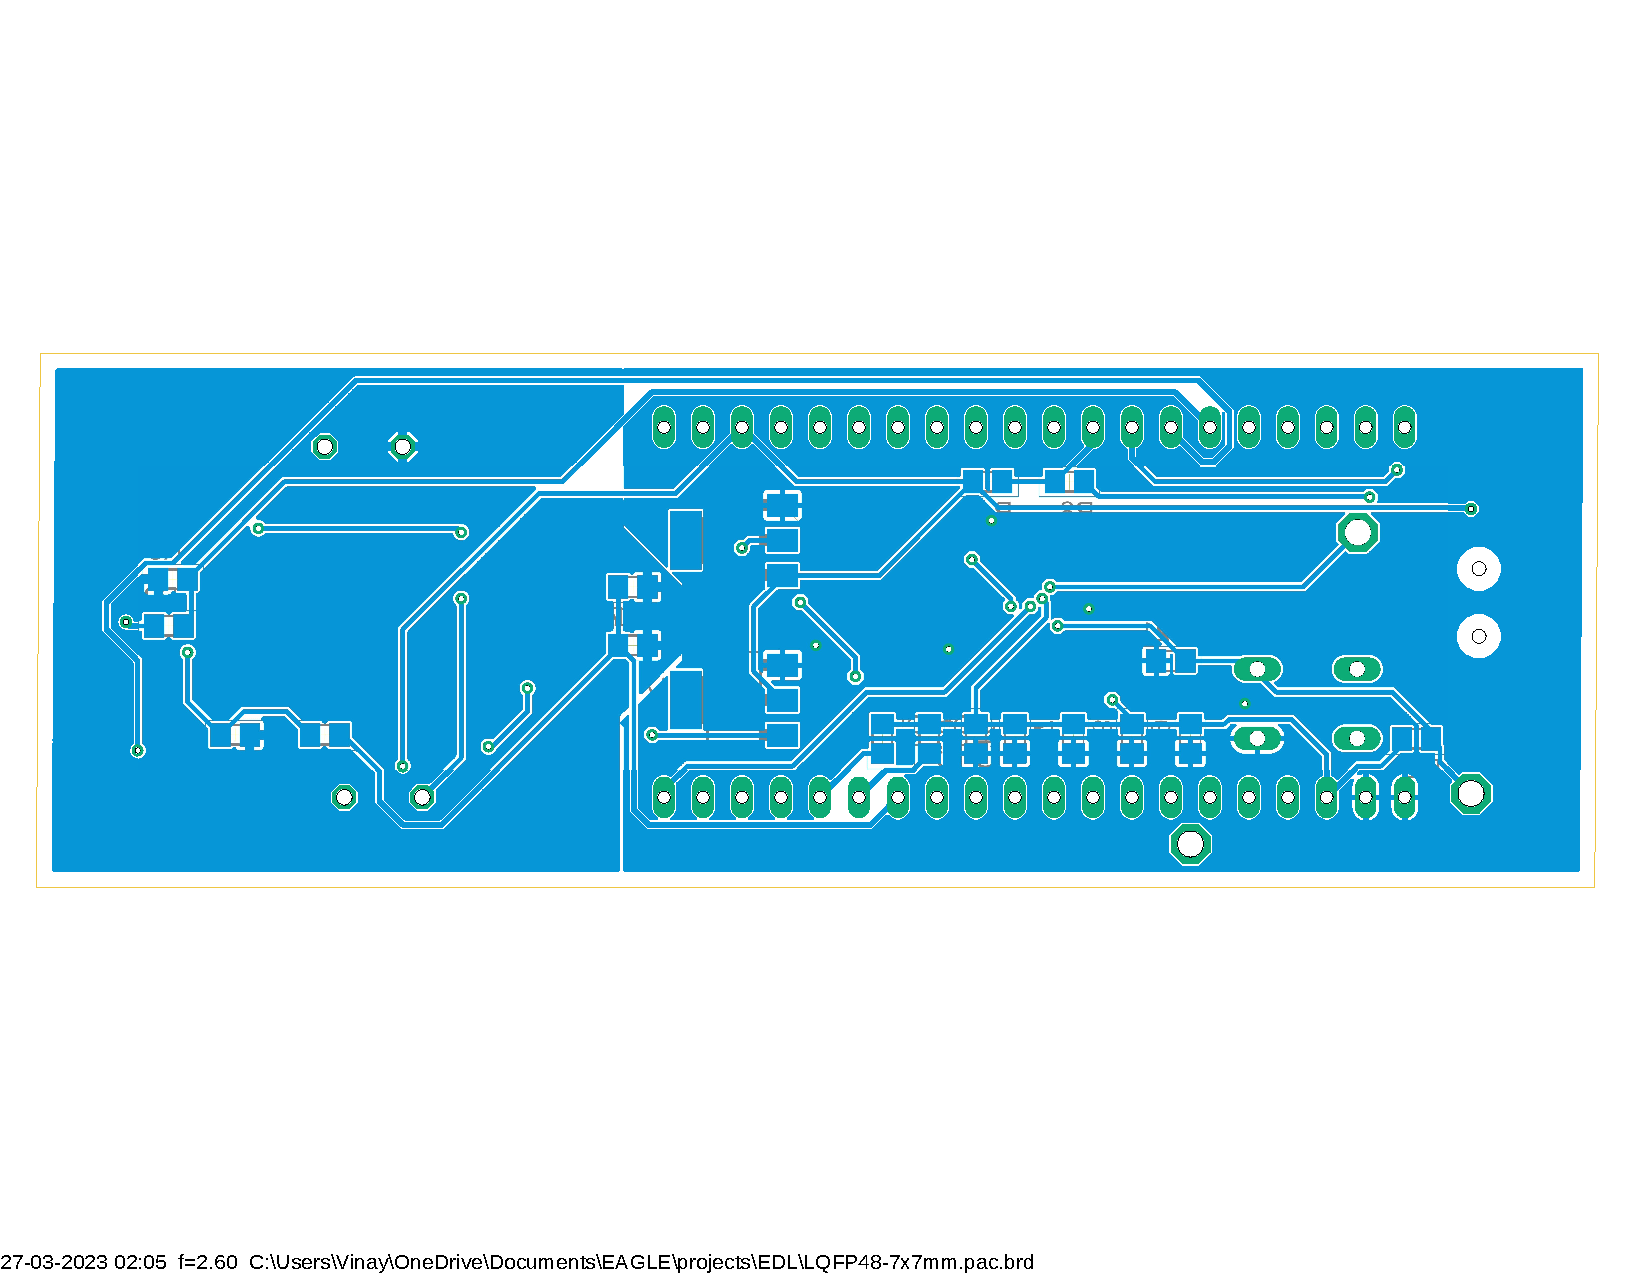
\includegraphics[width=\textwidth]{Images/ourpcbbottomgplane.pdf}
    \caption{PCB layout of bottom layer with ground plane}
    \label{fig:galaxy}
\end{figure}

\newpage


\section{Justification for component selection}
\subsection{Peltier Cell}
\textbf{Name- TEC1-12712.\\}
\textbf{Specifications - Qmax = 144W, Imax=12A} \\
Peltier with the above specifications was chosen because the one used in WELPCR had Imax=12A and Qmax=120W, so we decided to use Peltier with Qmax=144W so that samples can heat fast as it will have a high ramp rate. Other options are available, but their power rating is around 180W, and our supply rating is also 180W, so they might not be compatible as there are other components where this power will be distributed.


\begin{figure}[htp]
    \begin{subfigure}[b]{0.3\textwidth}
    \centering
    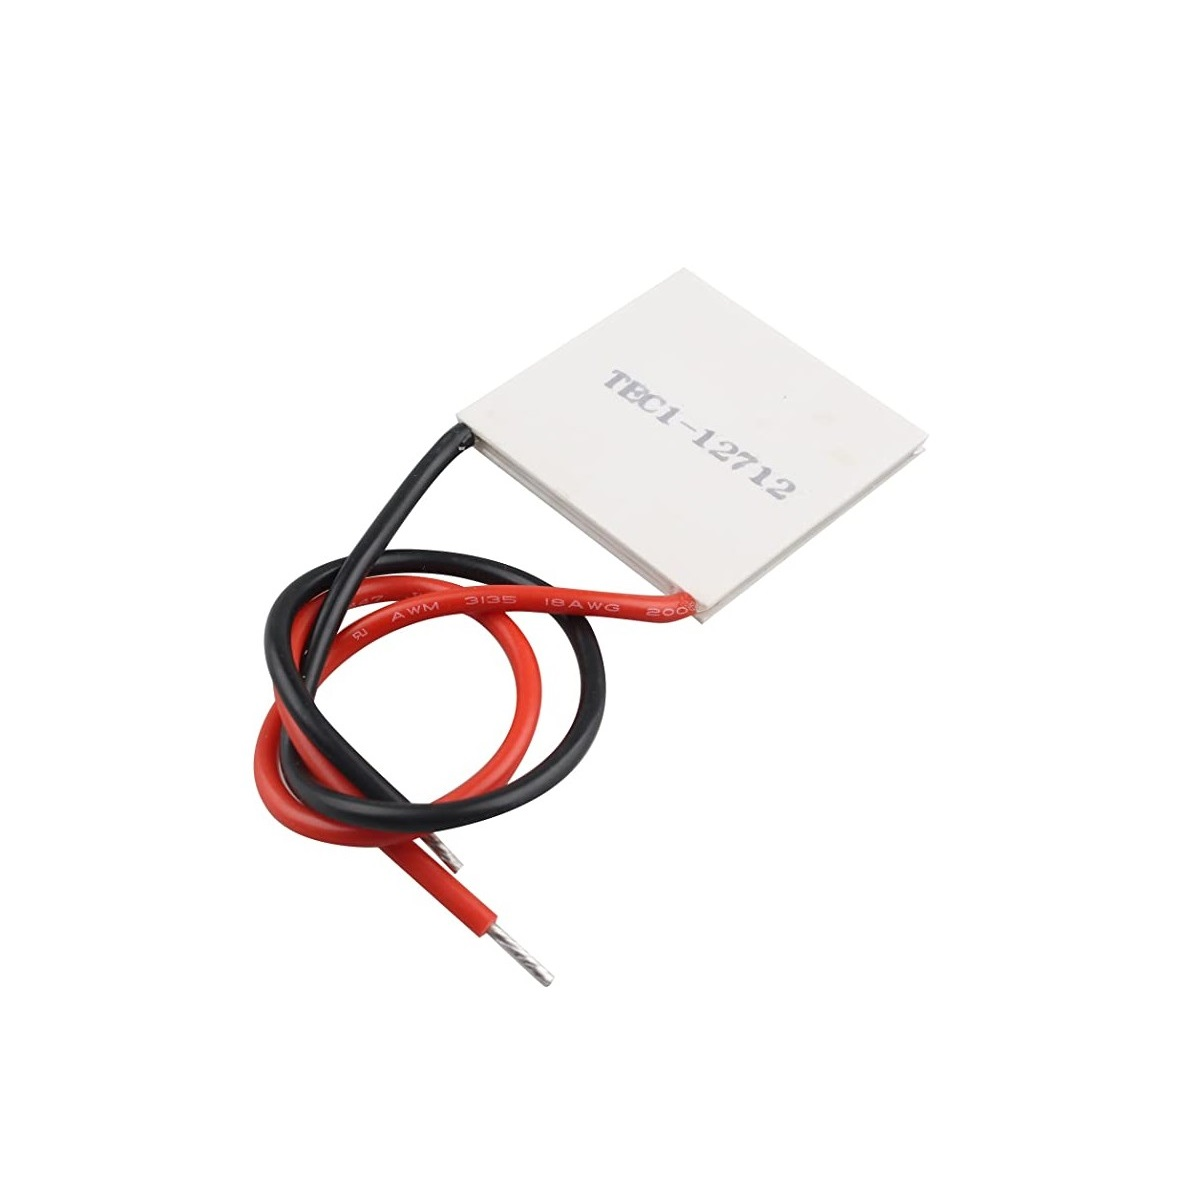
\includegraphics[width=\textwidth]{Images/peltier.jpg}
    \caption{Peltier cell}
    \end{subfigure}
    \hfill
    \begin{subfigure}[b]{0.3\textwidth}
        \centering
        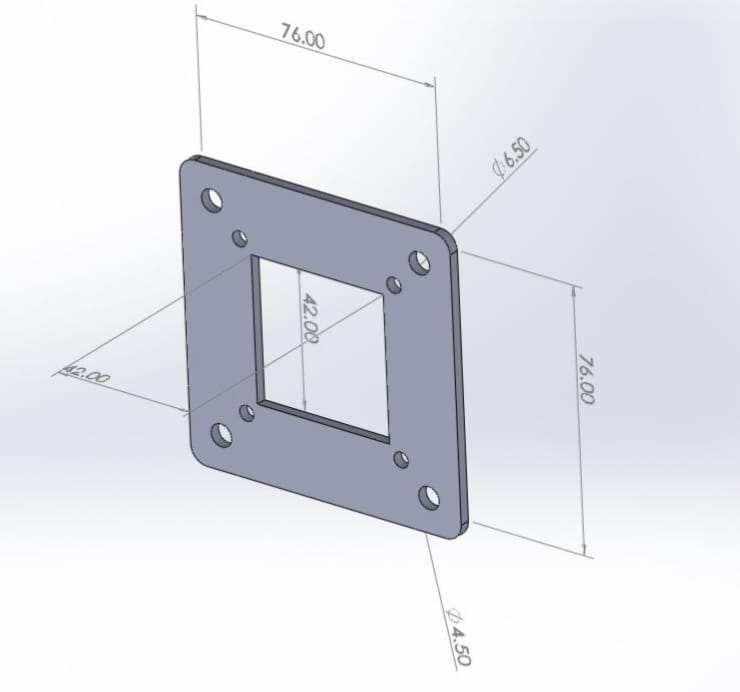
\includegraphics[width=\textwidth]{Images/Peltierbase2.jpeg}
        \caption{Peltier cell's isolation base}
    \end{subfigure}
    \hfill
    \begin{subfigure}[b]{0.3\textwidth}
        \centering
        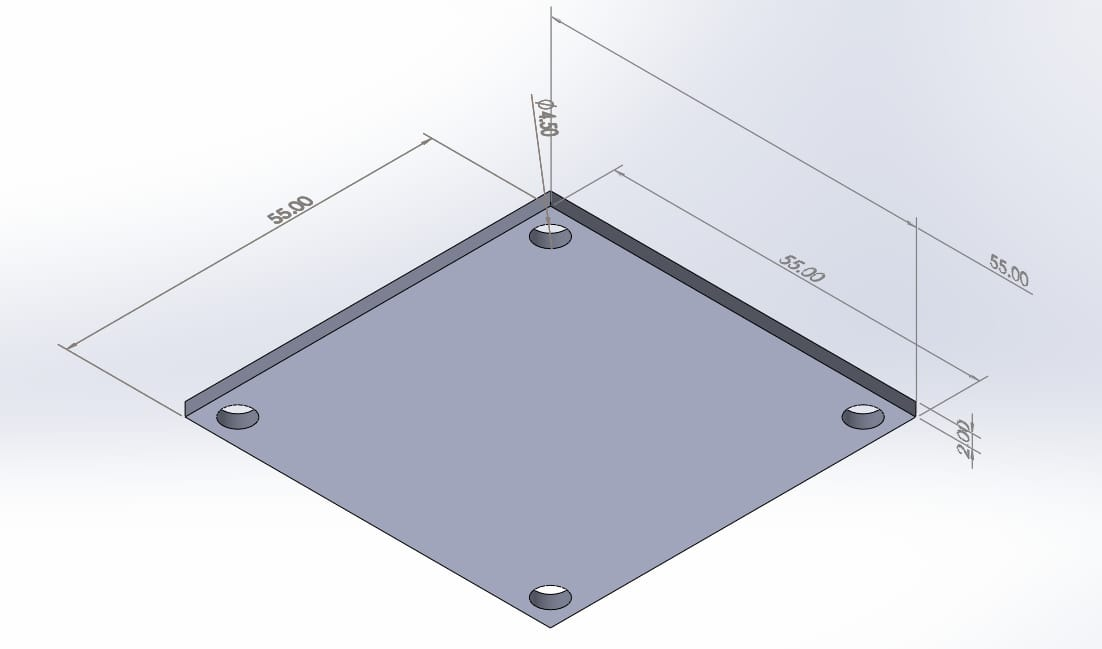
\includegraphics[width=\textwidth, height= 0.8\textwidth]{Images/peltierbase.jpeg}
        \caption{Base of the peltier cell}
    \end{subfigure}
    \caption{The Peltier cell: used for heating and cooling of the block}
    \label{fig:galaxy}
\end{figure}


\subsection{Microcontroller}
\textbf{Name- STM32F103C8T6}\\
This microcontroller satisfies our I/O requirements and was used in WELPCR also. It has 2 inbuilt 12 bit ADC's which will be helpful in reading the thermistor. It has 37 GPIO (General Purpose Input Output Pins) which will be sufficient for our requirement. Also the STM32F103C8T6 is widely used in various embedded systems applications such as robotics, industrial control, and home automation, among others.

\subsection{H-Bridge}
\textbf{VNH2SP30 Motor Driver}\\
It has an inbuilt H bridge to drive Peltier. The voltage range is between 5.5 to 16 Volts which satisfies our requirement. It is compatible with our microcontroller, and it can be controlled with PWM signals to control the speed and direction of the motor. It also has thermal shutdown and overcurrent protection.\\
Reference: https://www.instructables.com/Monster-Motor-Shield-VNH2SP30/


\subsection{Power Supply}
\textbf{Specifications - Qmax = 180W, Imax = 15A}\\
The Power Supply is appropriate for our component selection that is to drive the Peltier of 12A. Another option was to select a power supply of 12V 10A, but it won't be able to drive our Peltier. SMPS power supplies can provide precise regulation of the output voltage and current, which makes them suitable for use in sensitive electronic devices that require stable and clean power like our PCR Machine.

\subsection{Fan}
\textbf{Name- Silverstone KR02}\\
We plan to use the Silverstone KR02 fan as it has an rpm in the range of 800-2800, air flow rate 15.12~56.1 CFM which is better compared to Antec A30 which was used in WELPCR. Also, the dimensions are 97mm (W) x 125mm (H) x 51mm (D) compared to 125mm x 73mm x 86mm of Antec A30. This fan will help in the fast cooling to make the ramp rate better.


\begin{figure}[htp]
    \centering
    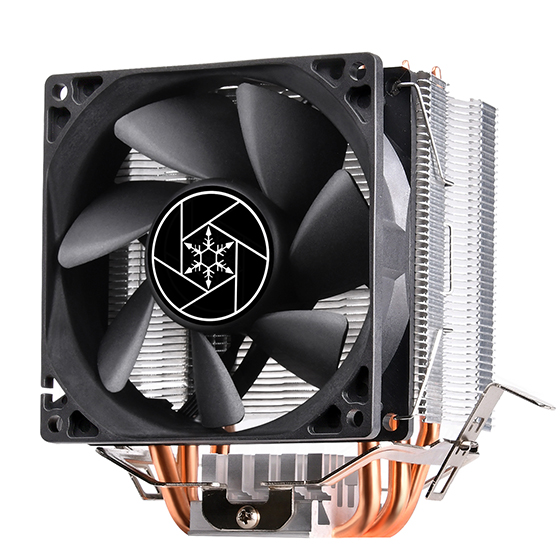
\includegraphics[width=4cm]{Images/fan.jpg}
    \caption{Silverstone KR02}
    \label{fig:galaxy}
\end{figure}


\subsection{Main Heating Block}
\textbf{Copper}\\
Copper is used for the main heating block instead of aluminium because it has a lower specific heat capacity (0.385) as compared to aluminium (0.89) thus will result in a faster heat transfer from the peltier to the wells which will give us a higher ramp rate. We have also reduced the size of the block to reduce the thermal mass of copper. The original block was of size 40x40 which we have reduced to make it 24x24.



\begin{figure}[htp]
    \centering
    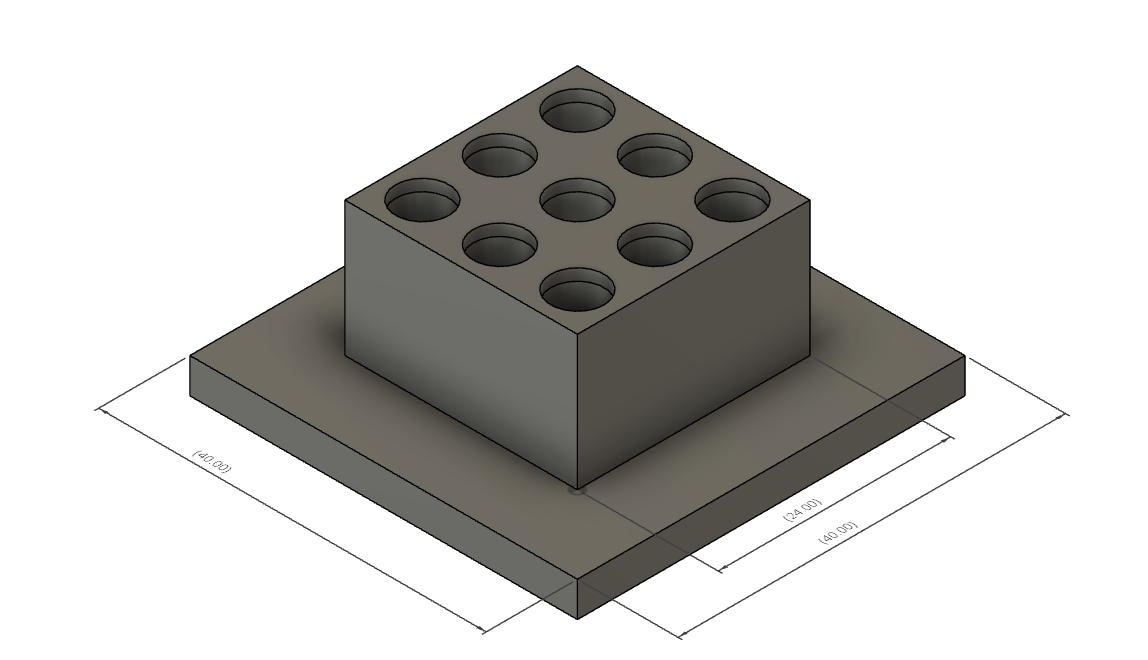
\includegraphics[width=10cm]{Images/Mainheatingblock.png}
    \caption{The main heating block created on autodesk fusion 360}
    \label{fig:galaxy}
\end{figure}




\maketitle

\section{Principle of operation of each subsystem}
\subsection{Heating Block}
The heating block is the component that holds the DNA sample and is responsible for heating the sample to the desired temperature. It is typically made of a thermally conductive material, such as aluminum, to ensure efficient heat transfer. But we use copper because it has a relatively higher thermal conductivity than aluminium. The heat is provided by the Peltier cell to the heating block.


\subsection{Cooling System}
The cooling system cools the DNA sample to the desired temperature. It can be a fan-based or refrigeration-based cooling system. We are using a fan-based system that will cool the DNA sample after the denaturation process in which the temperature rises to around 96. The peltier cell can act as a heat absorber if the direction of current is reversed in it. Thus, peltier is used for cooling of the main heating block.

\subsection{Temperature Controller}
The temperature controller measures the DNA sample's temperature and adjust the heating and cooling elements accordingly. It typically uses thermistors or thermocouples to measure the temperature and can be programmed to control the temperature profile for the PCR process. Here we will be using a thermistor ( Model : 20D-9 NTC ) to measure the temperature and then use the inbuilt ADC on the Micro-controller to control it. The sensors provide feedback to the heating and cooling system to ensure accurate temperature control during the PCR process.

\subsection{Heated Lid}
We would have a heated lid to cover the heating block to minimize condensation of the samples at the top of the sample tube and ensure that the there is no condensation of the sample on the upper side of the eppendorf tube. This heated lid is kept at a constant temperature of 100. Nichrome wire will be used in the heated lid for this purpose. We plan to follow the design of WELPCR for heated lid.



\begin{figure}[htp]
    \centering
    \begin{subfigure}[b]{0.4\textwidth}
    \centering
    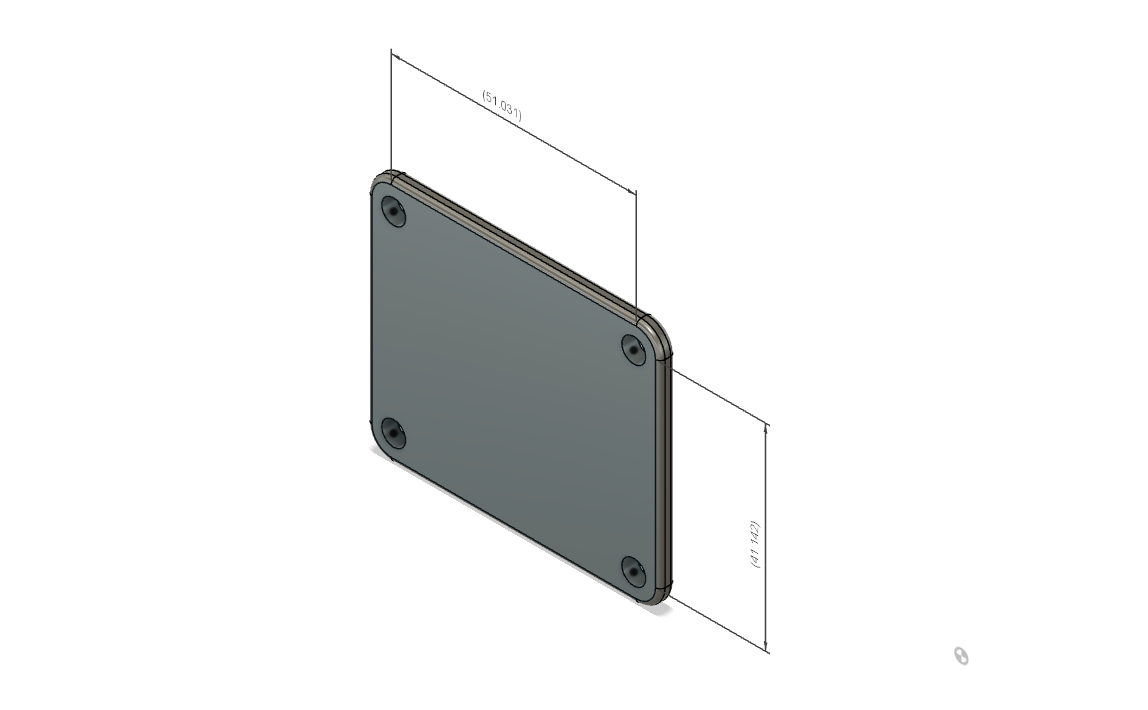
\includegraphics[width=7cm]{Images/Heatedlid1.png}
    \caption{Heating lid}
    \end{subfigure}
    \hfill
    \begin{subfigure}[b]{0.5\textwidth}
    \centering
    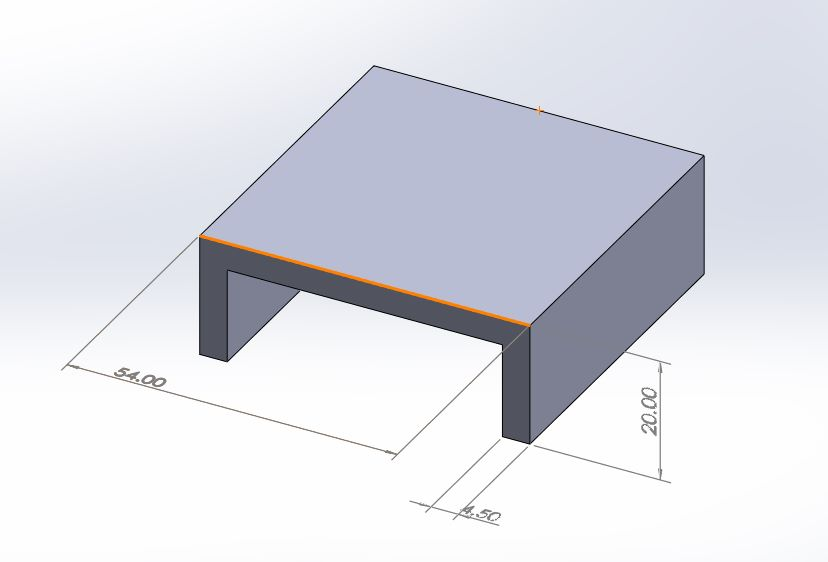
\includegraphics[width=7cm]{Images/heatinglid2.jpeg}
    \caption{Cover for heated lid}
    \end{subfigure}
    \caption{The heated lid model made on fusion 360}
    \label{fig:galaxy}
\end{figure}


\subsection{Control Unit}
The thermal cycler is controlled by a computer interface or control unit, which is used to program the temperature cycles and monitor the progress of the reaction. The control system is responsible for programming the thermal cycler, controlling the heating and cooling system, and monitoring the temperature of the reaction mixture. The control system uses a micro-controller to execute the PCR protocol and provide feedback to the user.

\subsection{Power Supply}
A power supply is used to power the PCR machine's various components, including the micro-controller, heating element ( Peltier Cell ), and cooling element ( Fan ). It would be connected to the micro-controller for controlling the voltage and current. H-Bridge is used to reverse the direction of current in order to decide whether we want to heat or cool the sample.

\subsection{H-Bridge}
The H-Bridge is used to switch the current through the peltier that is in thermal contact with the sample. By switching the current through the heating element on and off in a precise manner, the temperature of the sample can be raised or lowered rapidly and accurately to the desired temperature for the various steps of the PCR process.


\subsection{LCD Display}
The results of the PCR Machine will be shown on an LCD screen. The results include the running time along with the controllability of time of reaction. The graphs for the current ongoing PCR machine will also be displayed and we can input the number of cycles for which we want to perform the PCR reaction.


\maketitle


\section{ Preliminary analysis }

The Copper Block has been given for manufacturing post which the following experiment will be conducted:
\begin{itemize}

\item Aim: To check the copper block prepared.
\item Method: The copper block prepared by us will be installed on the already existing WELPCR. Then the PCR process will be started on the machine to check the ramp rate obtained. The ramp rate will be observed from the LCD.
\item Results:  After seeing the ramp rate, it will be decided whether to use the formed copper block for further use or not.
\item Next Step: If the desired ramp rate is not observed then other design of blocks like trapezium shaped block to have max heat transfer.

\end{itemize}
\maketitle
\newpage
\section{Mechanical Designs}

One of the major components of mechanical designing was to make an appropriate heating block so as to minimize the thermal mass and maximize the heat transfer. So here we greatly reduced the size of the thermal block and reduced the gap between samples for faster heat transfer and lower loss of heat.


\begin{figure}[htp]
    \centering
    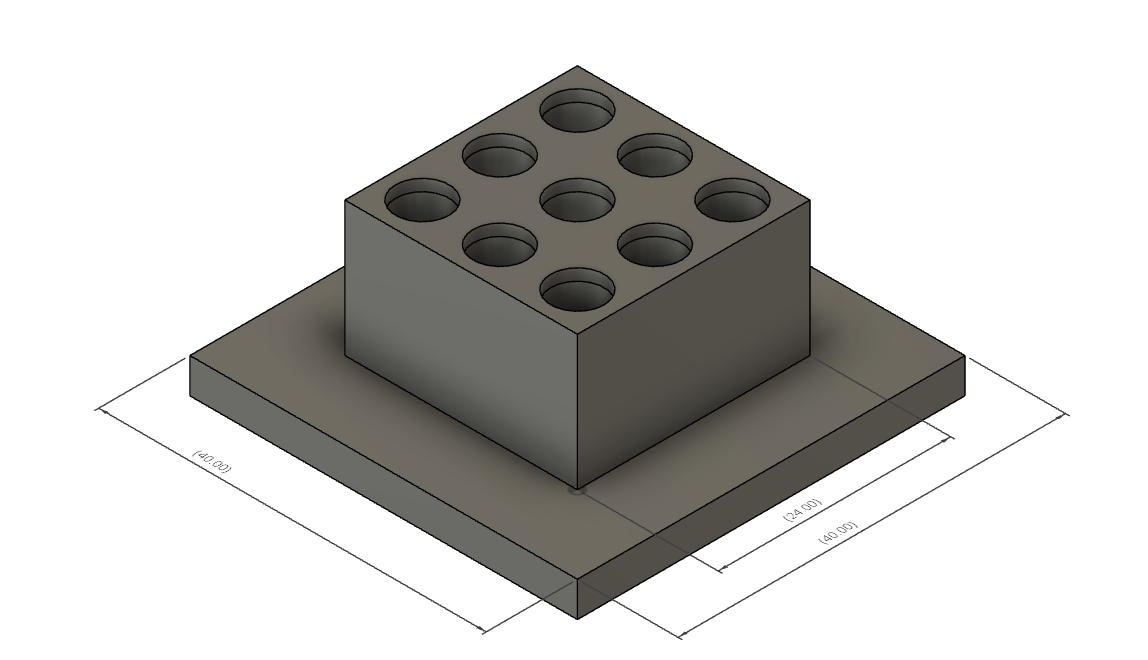
\includegraphics[width=9cm]{Images/Mainheatingblock.png}
    \caption{The main heating block created on autodesk fusion 360}
    \label{fig:galaxy}
\end{figure}




The depth of the samples were calculated using the tube dimensions and it's mechanical design. Help was taken from the RA and TA for this design and dimension calculation.


\begin{figure}[htp]
    \centering
    \begin{subfigure}[b]{0.4\textwidth}
    \centering
    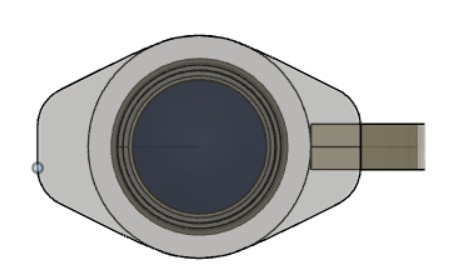
\includegraphics[width=5cm]{Images/Tubetop.jpeg}
    \caption{Top View of Tube}
    \end{subfigure}
    \hfill
    \begin{subfigure}[b]{0.5\textwidth}
    \centering
    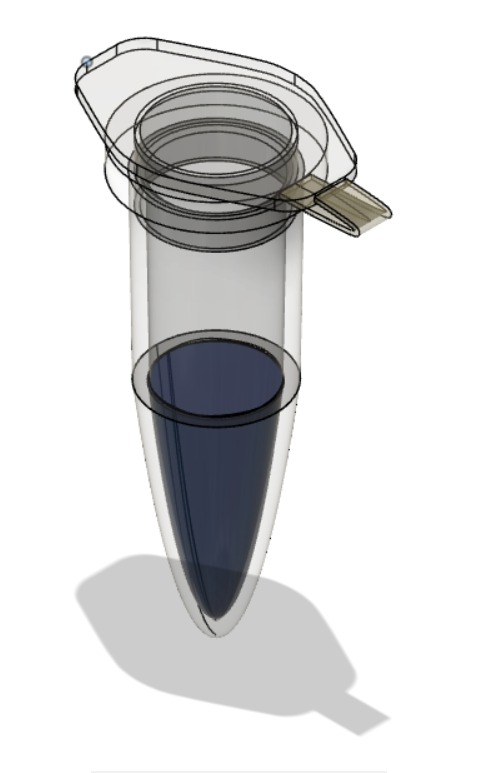
\includegraphics[width=5cm]{Images/Tubeside.jpeg}
    \caption{Side View of Tube}
    \end{subfigure}
    \caption{Tube for putting samples}
    \label{fig:galaxy}
\end{figure}

\newpage
Another component that we have is the heated lid at the top of the Peltier cell which will be maintained at a constant temperature of around 100 to prevent condensation and this will be made of aluminium as given below :\\


\begin{figure}[htp]
    \centering
    \begin{subfigure}[b]{0.4\textwidth}
    \centering
    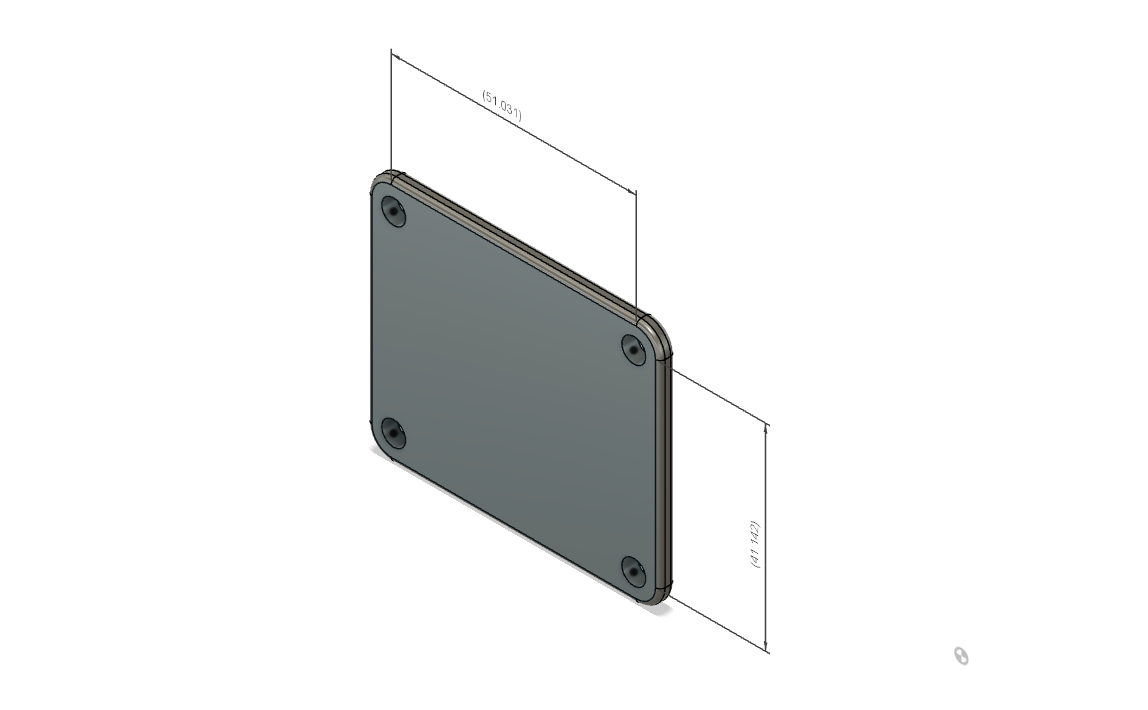
\includegraphics[width=7cm]{Images/Heatedlid1.png}
    \caption{Heating lid}
    \end{subfigure}
    \hfill
    \begin{subfigure}[b]{0.5\textwidth}
    \centering
    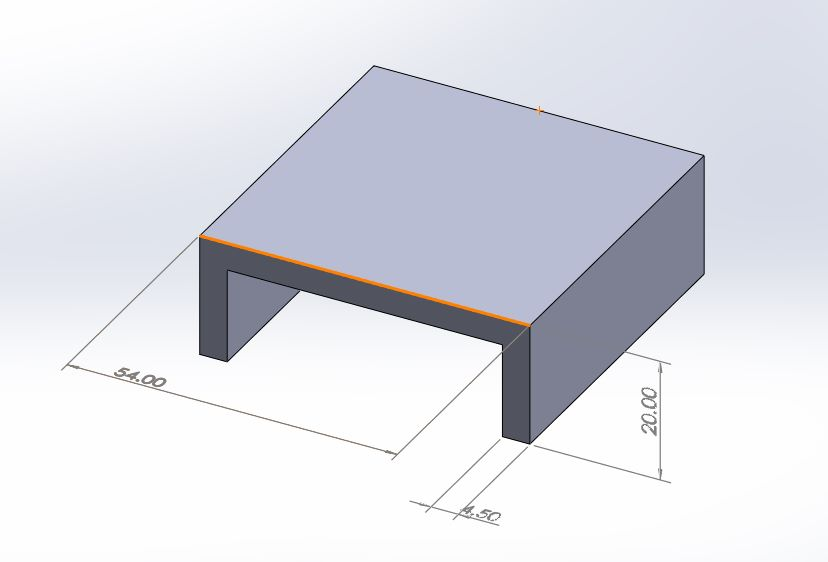
\includegraphics[width=7cm]{Images/heatinglid2.jpeg}
    \caption{Cover for heated lid}
    \end{subfigure}
    \caption{The heated lid model made on fusion 360}
    \label{fig:galaxy}
\end{figure}

We also need to design a \textbf{base} for Peltier on which it can rest. It's a 3-layer system which will be as shown below:


\begin{figure}[htp]
    \centering
    \begin{subfigure}[b]{0.4\textwidth}
    \centering
    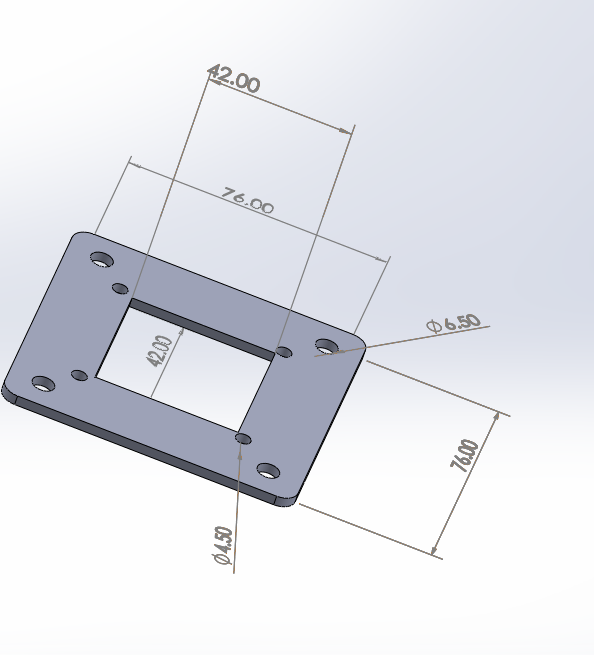
\includegraphics[width=5cm]{Images/Isolation_Base.png}
    \caption{Base Top View}
    \end{subfigure}
    \hfill
    \begin{subfigure}[b]{0.5\textwidth}
    \centering
    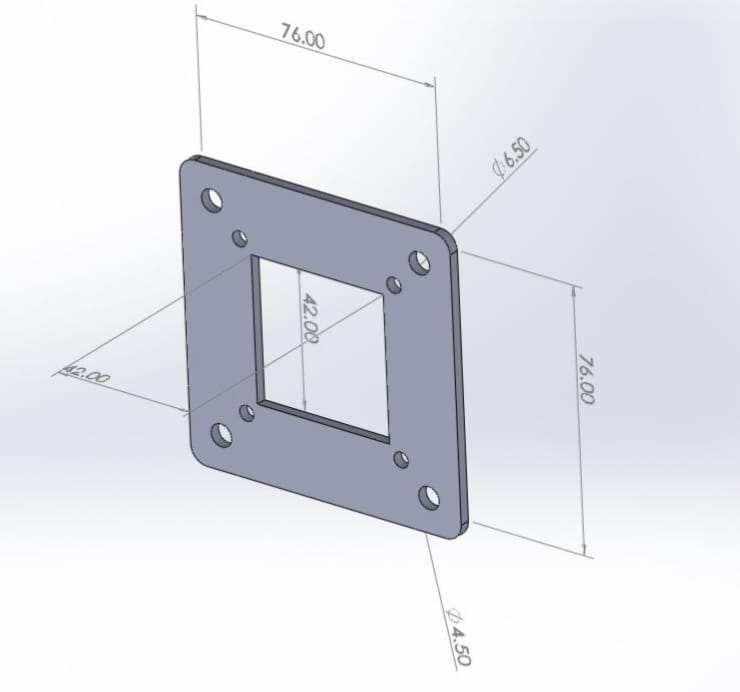
\includegraphics[width=5cm]{Images/Peltierbase2.jpeg}
    \caption{Base Side View}
    \end{subfigure}
    \caption{The heated lid model made on fusion 360}
    \label{fig:galaxy}
\end{figure}




Below this plate, we have a \textbf{Peltier cover} which is around the same size and below which, again, a \textbf{metal plate} of almost same size as Peltier is used the design for which is given as :

\begin{figure}[h]
    \centering
    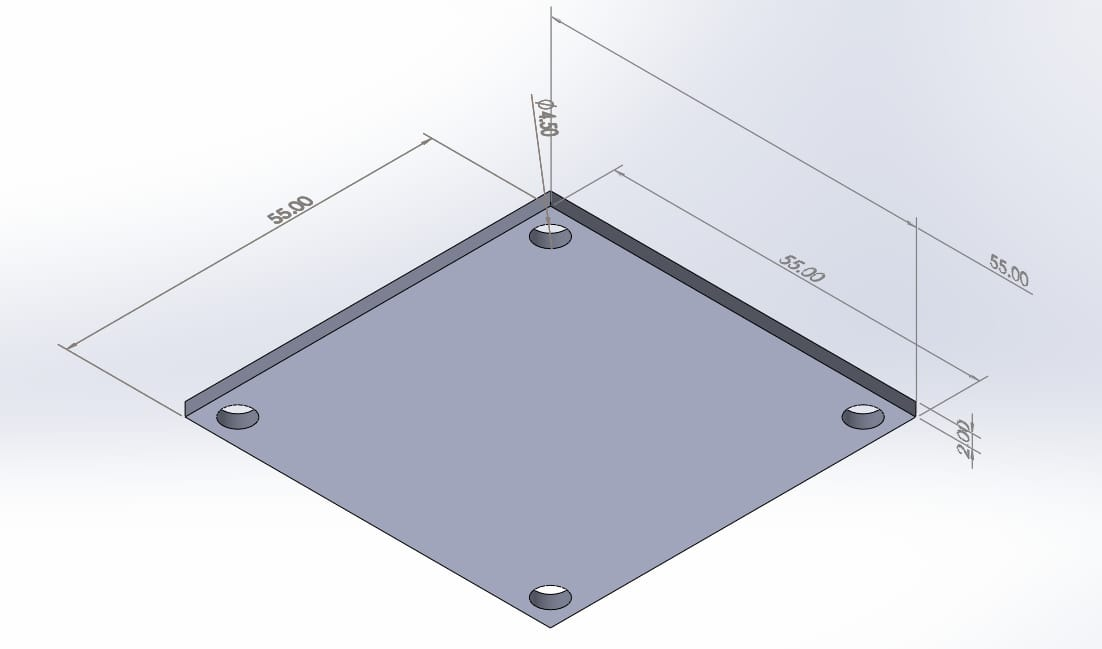
\includegraphics[width=7cm]{Images/peltierbase.jpeg}
    \caption{The main heating block created on autodesk fusion 360}
    \label{fig:galaxy}
\end{figure}

\pagebreak

\section{CAD Design}
Following are the CAD designs for the laser cutting of the outer casing of PCR Machine.
\begin{figure}[h]
    \centering
    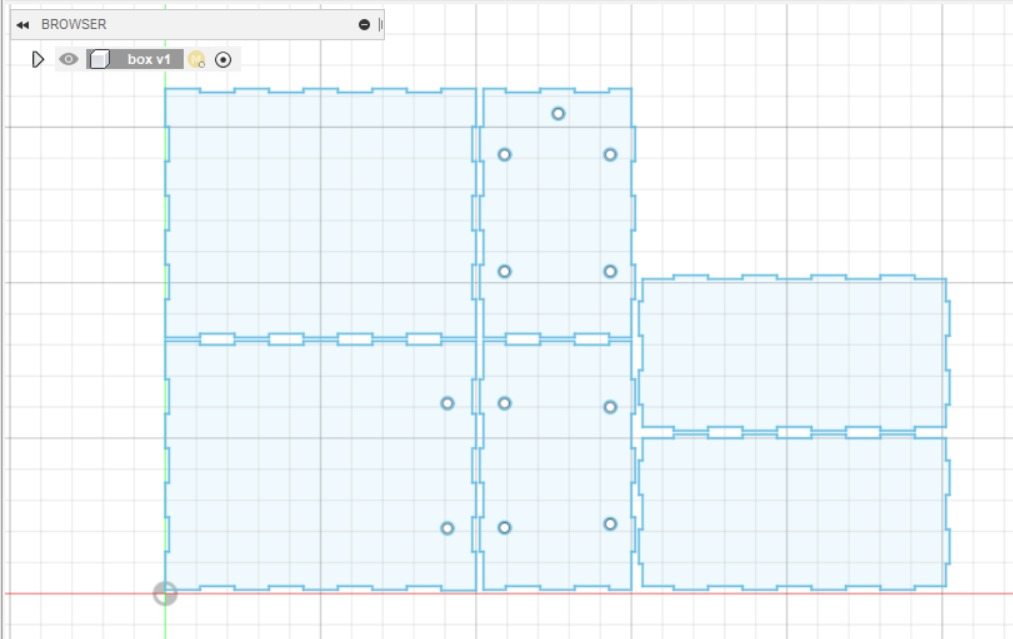
\includegraphics[width=9cm]{casing 2d.jpeg}
    \caption{2D design of outer casing}
    \label{fig:galaxy}
\end{figure}

\begin{figure}[h]
    \centering
    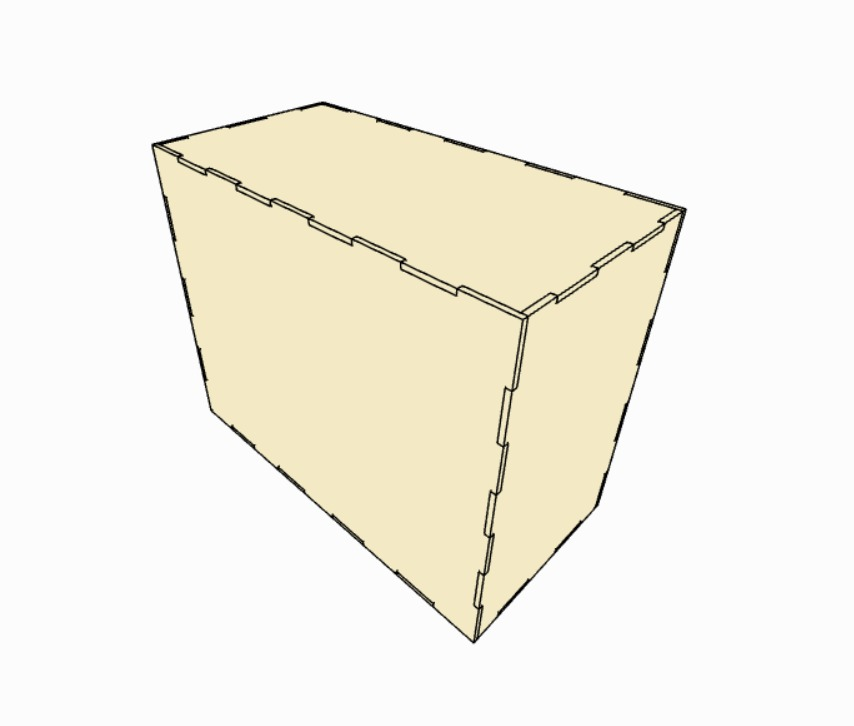
\includegraphics[width=7cm]{casing 3d.jpeg}
    \caption{3D design of outer casing}
    \label{fig:galaxy}
\end{figure}

\begin{figure}[h]
    \centering
    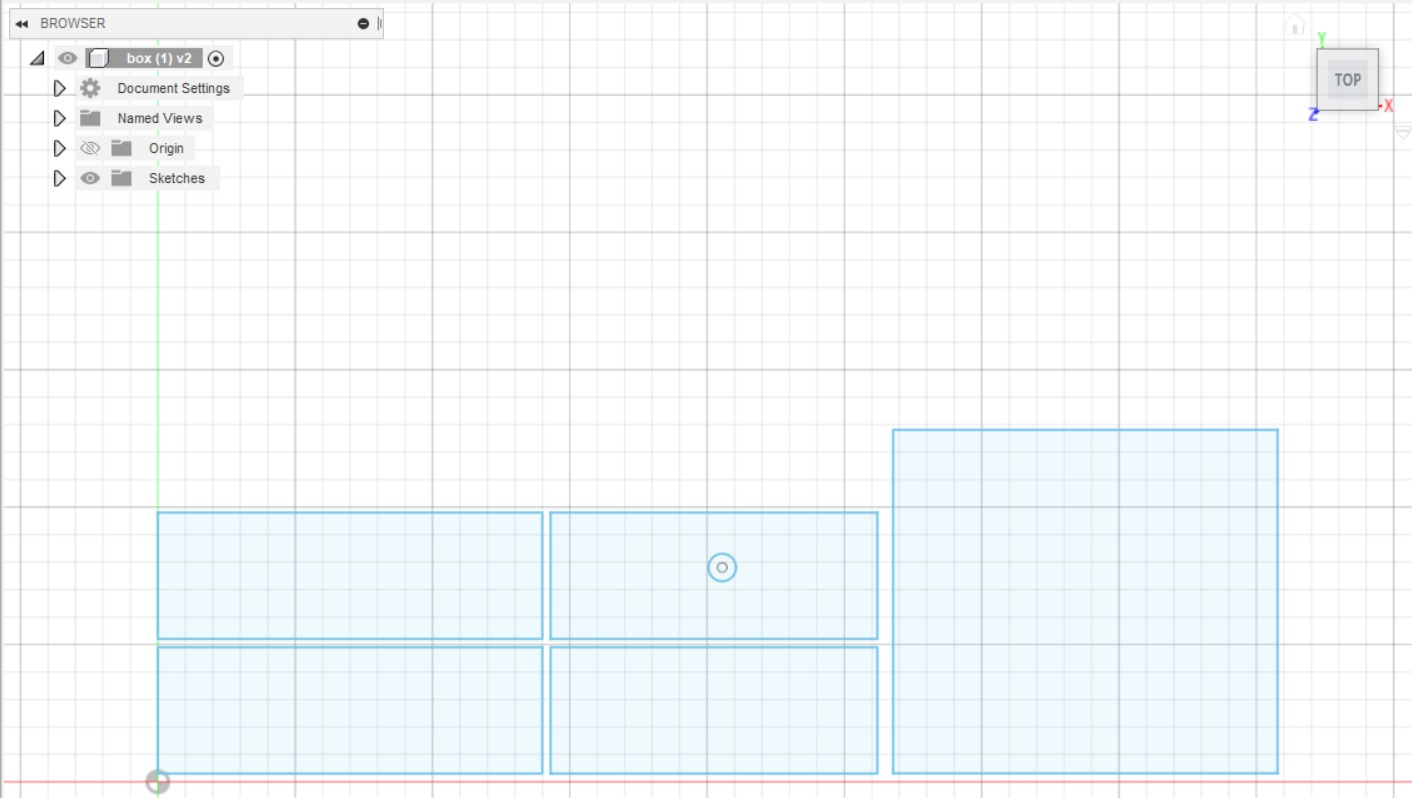
\includegraphics[width=7cm]{lid 2d.jpeg}
    \caption{2D design of lid cover}
    \label{fig:galaxy}
\end{figure}

\begin{figure}[h]
    \centering
    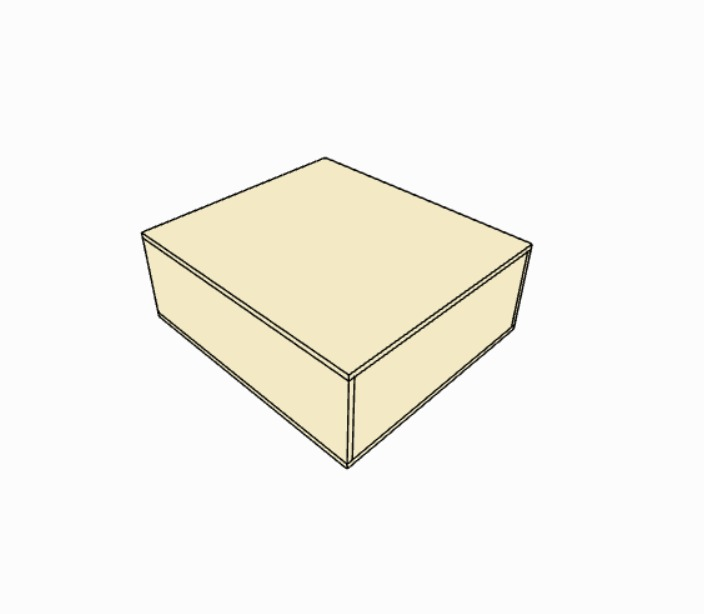
\includegraphics[width=7cm]{lid 3d.jpeg}
    \caption{3D design of lid casing}
    \label{fig:galaxy}
\end{figure}


\maketitle
\section{Testing of Sub-Circuits}
\subsubsection{Voltage Regulator(12V to 5V)}

\begin{figure}[h]
    \centering
    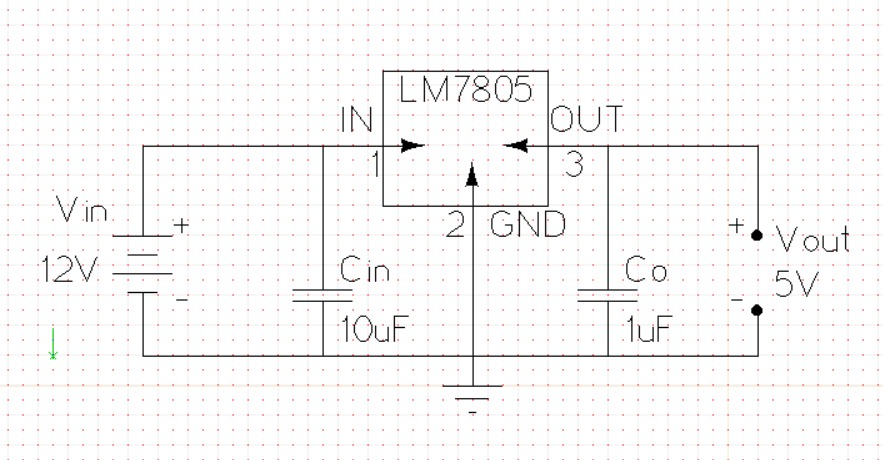
\includegraphics[width=7cm]{lm7805.jpeg}
    \caption{Circuit used for Testing Voltage Regulator(12V to 5V)}
    \label{fig:galaxy}
\end{figure}


We did the testing for the Voltage Regulator(LM7805C), which will convert the input voltage of 12V to 5V to be supplied to the USB, and it seemed to work fine.
Here is the snapshot of the circuit.

\begin{figure}[h]
    \centering
    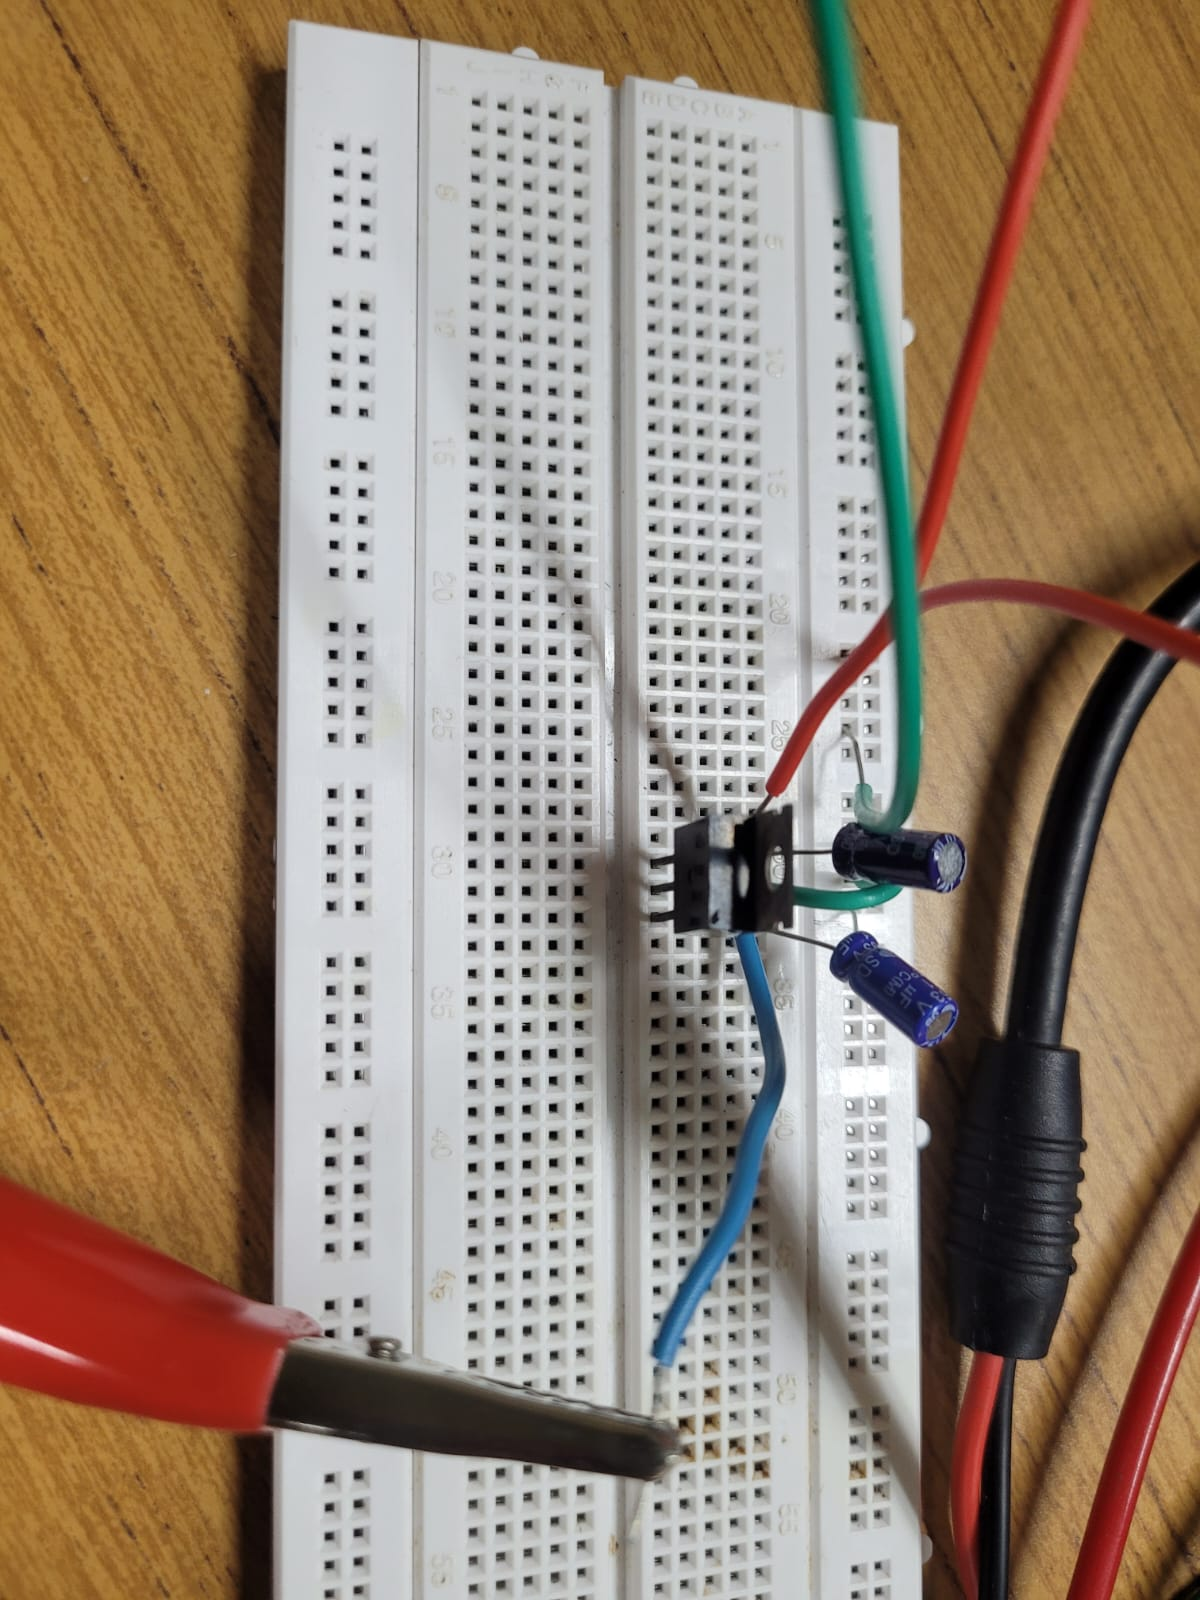
\includegraphics[width=7cm]{Voltage_regulator2.jpeg}
    \caption{Circuit used for Testing Voltage Regulator}
    \label{fig:galaxy}
\end{figure}
\begin{figure}[h]
    \centering
    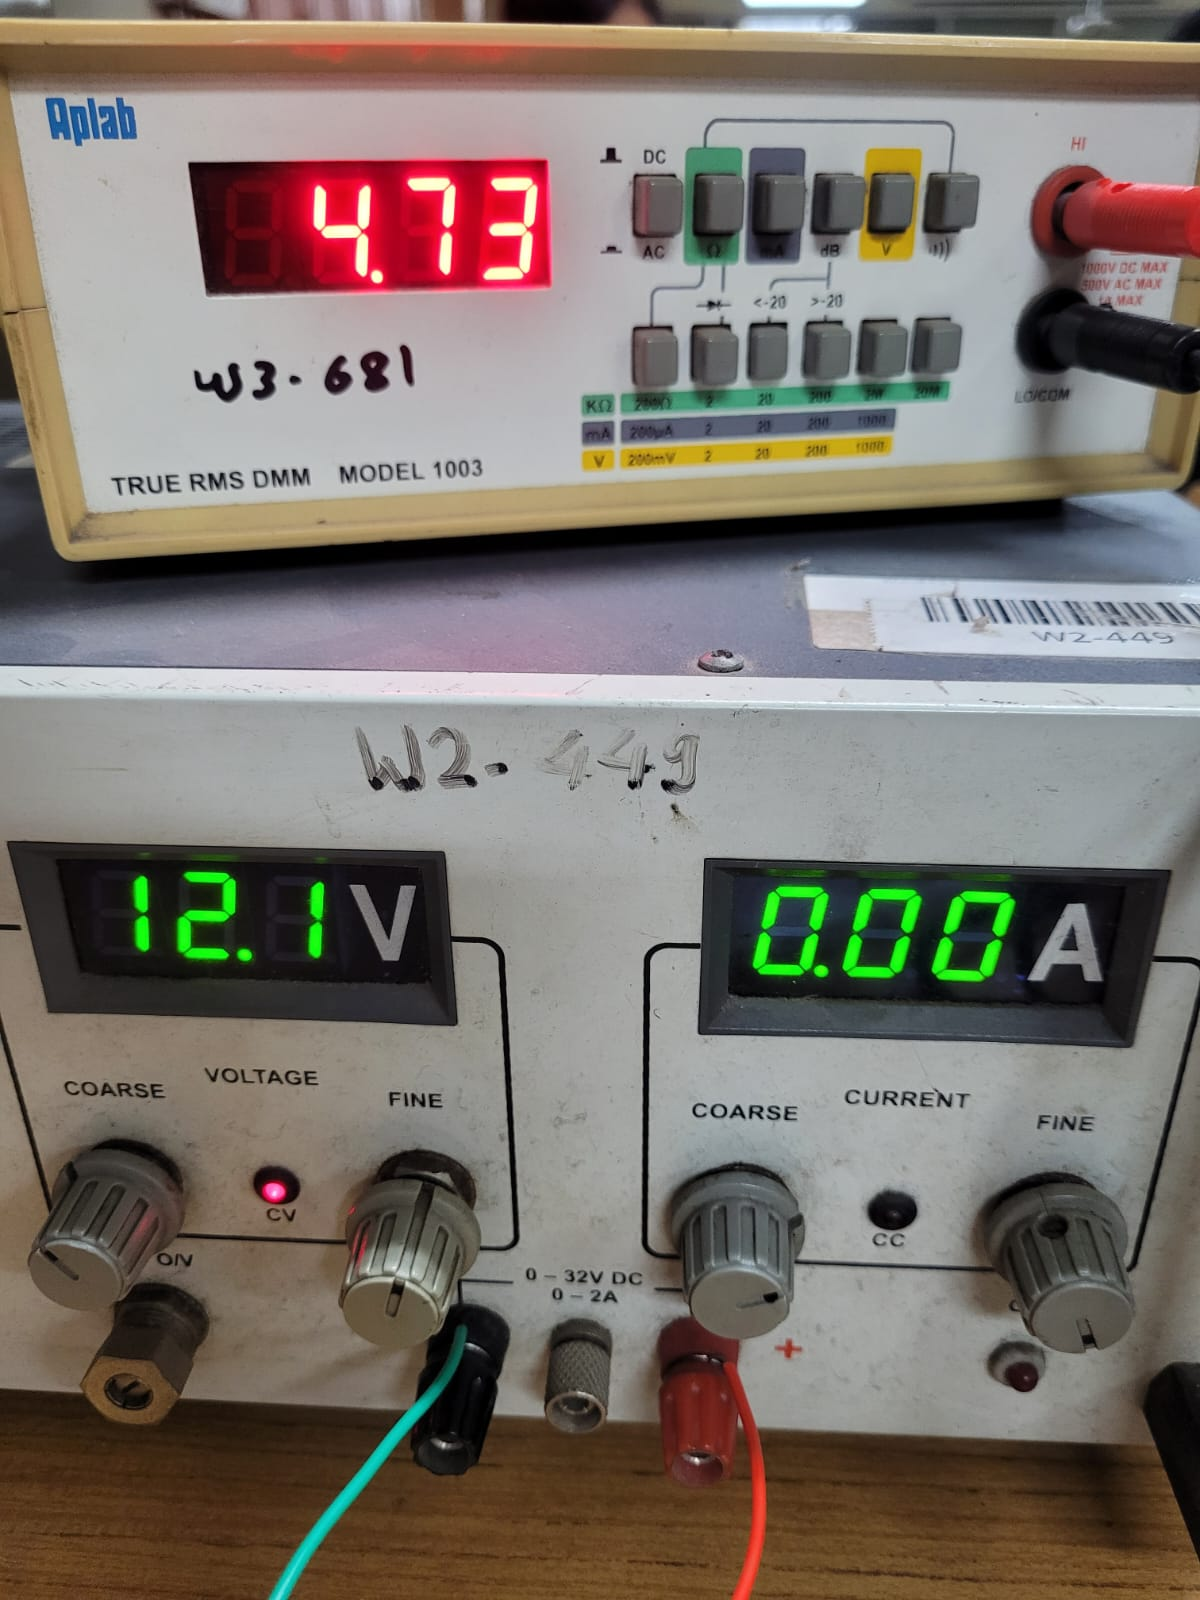
\includegraphics[width=7cm]{Voltage_regulator1.jpeg}
    \caption{Output Voltage from Voltage Regulator}
    \label{fig:galaxy}
\end{figure}

\subsubsection{Voltage Regulator 5V to 3.3V}
Below is the circuit for the Voltage regulator that takes 5V input and gives 3.3V output to be used by the microcontroller.


\begin{figure}[h]
    \centering
    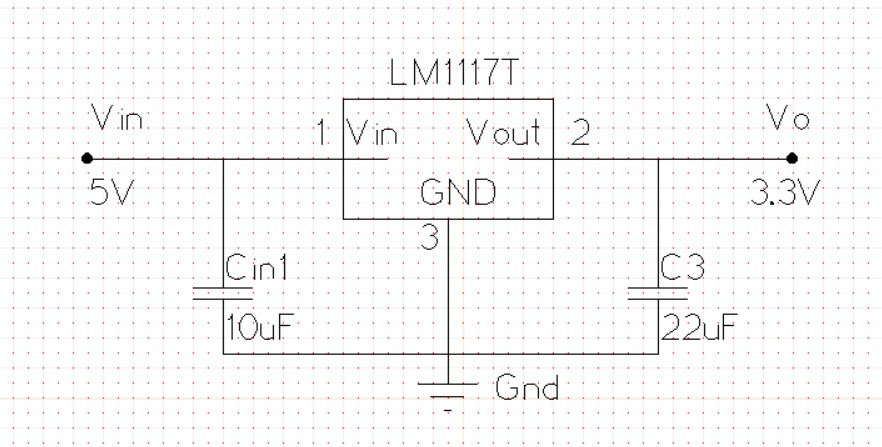
\includegraphics[width=7cm]{Voltage regulator.jpeg}
    \caption{Voltage Regulator(5V to3.3V}
    \label{fig:galaxy}
\end{figure}


\section{Programming}

\subsubsection{Code for interfacing of \textbf{Thermistor} with \textbf{STM32F103C8T6}}
We have written the code for interfacing the thermistor with the microcontroller to sense temperature from Peltier and send the signal to the microcontroller and display the temperature on LCD.
Here is the screenshot of the above-mentioned Program


\begin{figure}[h]
    \centering
    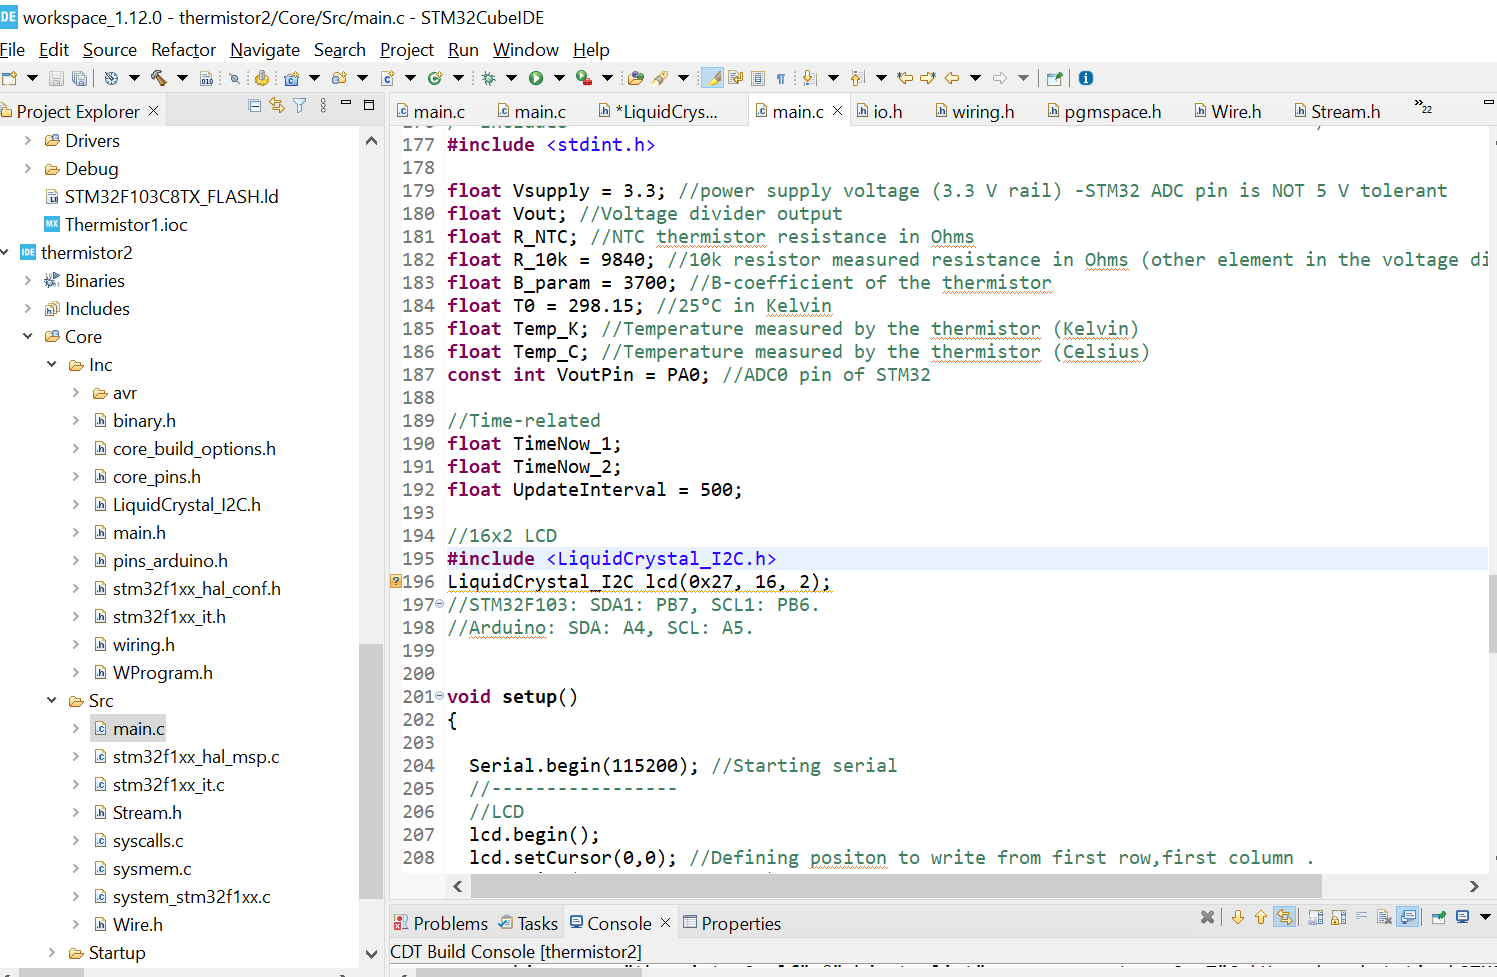
\includegraphics[width=10cm]{Code1.png}
    \caption{Code for Thermistor}
    \label{fig:galaxy}
\end{figure}
\begin{figure}[h]
    \centering
    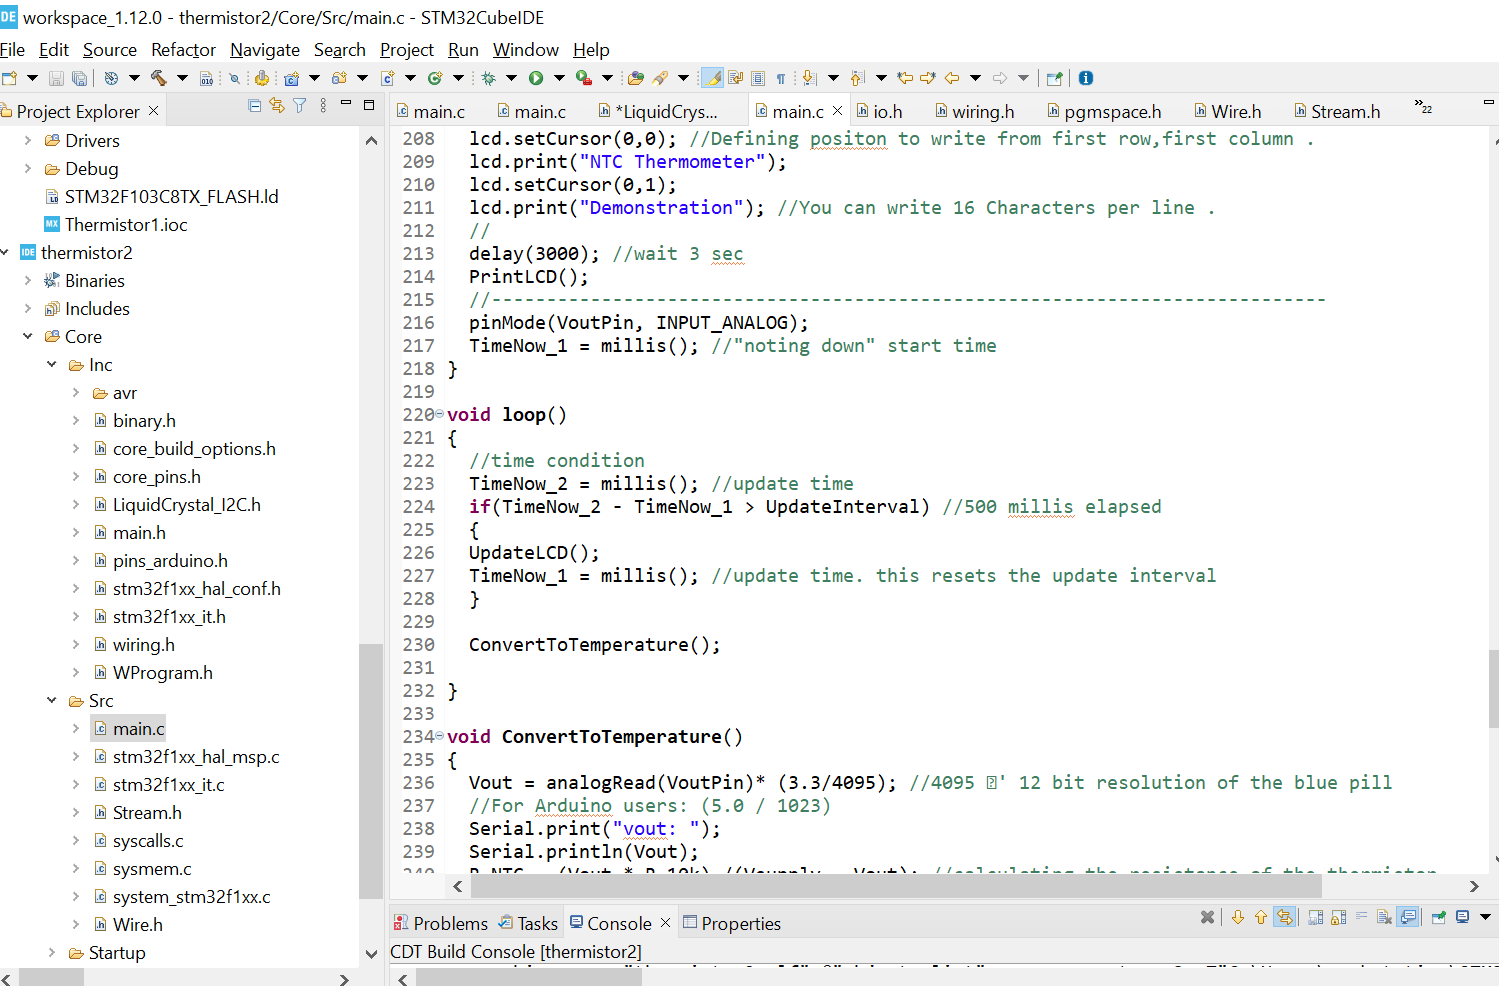
\includegraphics[width=10cm]{Code2.png}
    \caption{Code for Thermistor}
    \label{fig:galaxy}
\end{figure}
\begin{figure}[h]
    \centering
    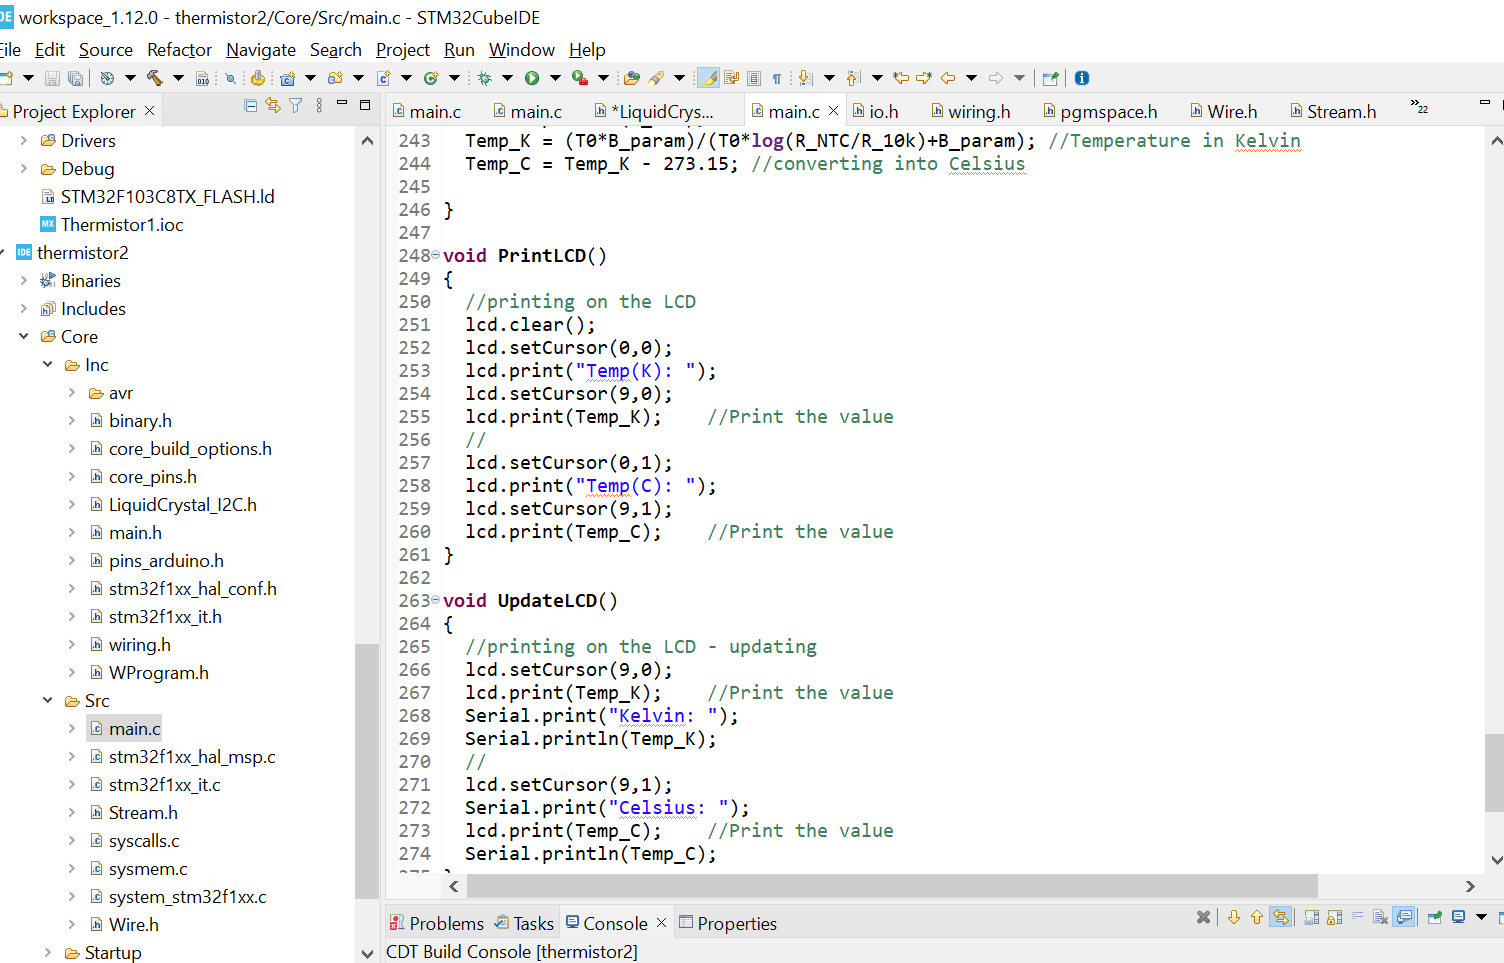
\includegraphics[width=10cm]{Code3.png}
    \caption{Code for Thermistor}
    \label{fig:galaxy}
\end{figure}
\begin{figure}[h]
    \centering
    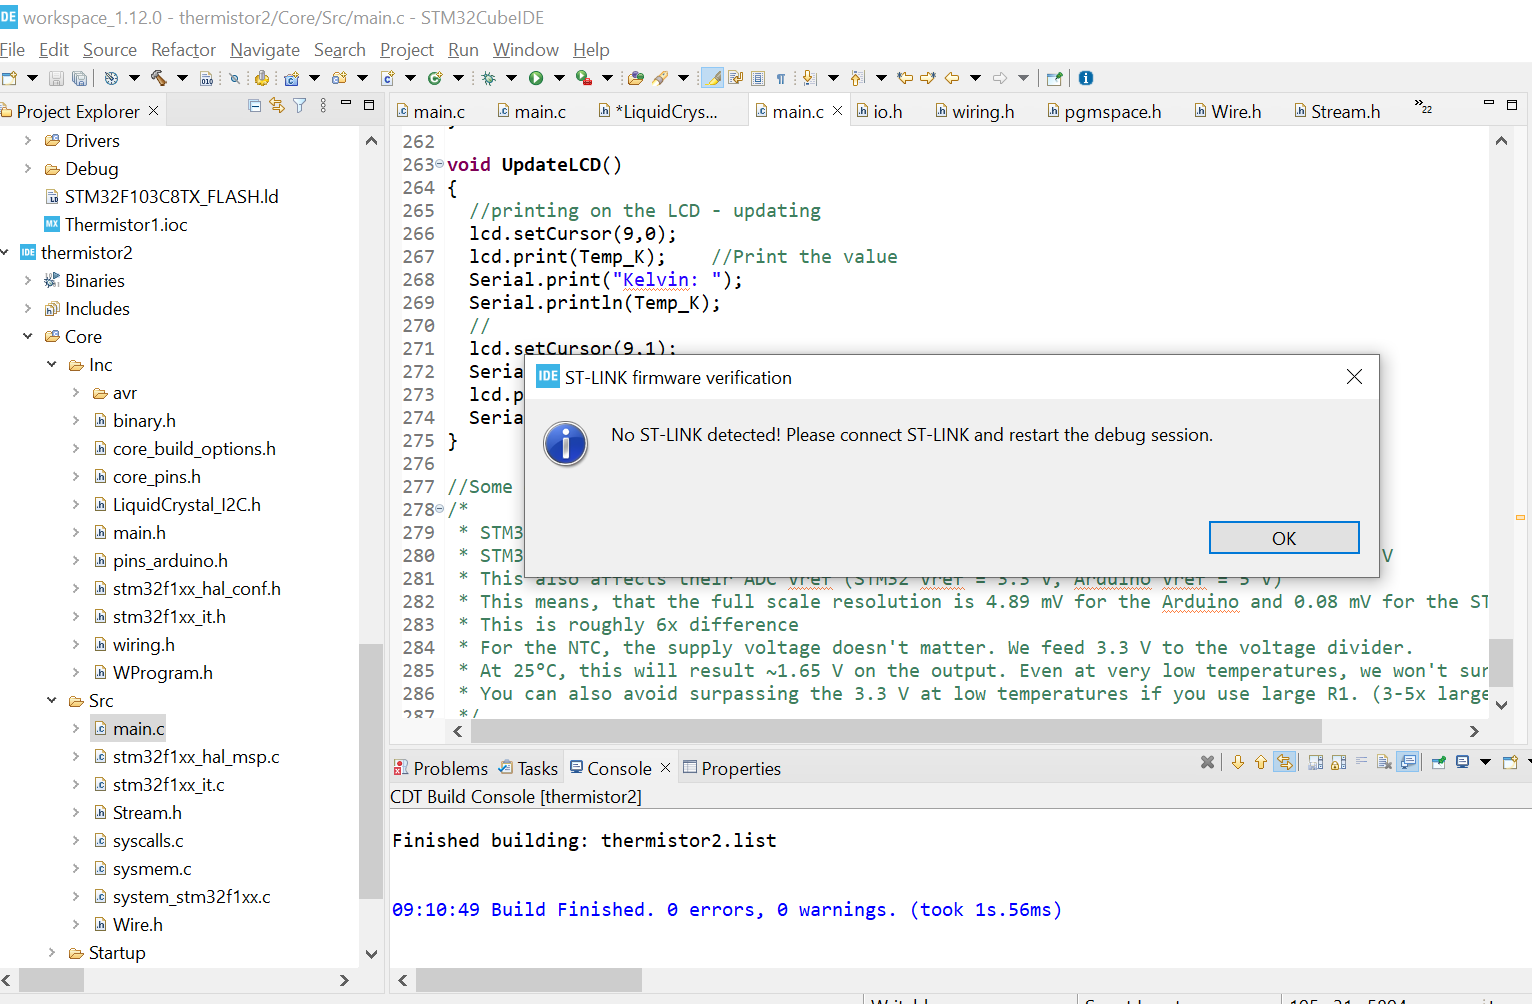
\includegraphics[width=10cm]{Code4.png}
    \caption{Code compiled with 0 errors and is ready to be used for interfacing}
    \label{fig:galaxy}
\end{figure}
\section{Risk mitigation/contingency}
\subsection{Ramp rate not achieved}
\begin{itemize}
    \item \textbf{Anticipated problem}: The copper block has better thermal conductivity than aluminum but has more thermal mass, so it may require more power to achieve the required ramp rate.
\item \textbf{Likelihood}: High
\item \textbf{Mitigation strategy}: We plan to test it on WELPCR, and if the ramp rate is not achieved, then we will try using an aluminium block or with another design for the copper block.
\end{itemize}

\subsection{Possibility of short circuit and overcurrent}
\begin{itemize}
    \item 
\textbf{Anticipated problem}: Our circuit uses high currents and the microcontroller has a maximum current rating of 150mA. This may cause damage to components.
\item \textbf{Likelihood}: High
\item \textbf{Mitigation strategy}: Creating overcurrent and overvoltage detection circuits and applying proper spacing in PCB.
\end{itemize}
\subsection{Heating of conducting wires}
\begin{itemize}
    \item 
\textbf{Anticipated problem}: High current and heating block may cause the melting of wires or damage to components.
\item \textbf{Likelihood}: Medium
\item \textbf{Mitigation strategy}: We plan to cover this during the packaging of the circuit.
\end{itemize}

\end{document}
